% ============================================================
%  Nassau Candy Distributor — Supply Chain Analytics
%  Research Paper — LaTeX Source
% ============================================================
\documentclass[12pt, a4paper]{article}

% ---------- Packages ----------
\usepackage[margin=1in]{geometry}
\usepackage{setspace}
\usepackage{titlesec}
\usepackage{booktabs}
\usepackage{array}
\usepackage{tabularx}
\usepackage{longtable}
\usepackage{multirow}
\usepackage{graphicx}
\usepackage{float}
\usepackage{subcaption}
\usepackage{caption}
\usepackage{amsmath}
\usepackage{amssymb}
\usepackage{hyperref}
\usepackage{xcolor}
\usepackage{enumitem}
\usepackage{fancyhdr}
\usepackage{abstract}
\usepackage[authoryear, round]{natbib}
\usepackage{microtype}
\usepackage{parskip}
\usepackage{listings}
\usepackage{colortbl}
\usepackage[T1]{fontenc}
\usepackage{lmodern}

% ---------- Hyperlink setup ----------
\hypersetup{
    colorlinks=true,
    linkcolor=blue!60!black,
    citecolor=blue!60!black,
    urlcolor=blue!60!black,
}

% ---------- Header / Footer ----------
\pagestyle{fancy}
\fancyhf{}
\rhead{\small Nassau Candy Distributor --- Supply Chain Analytics}
\lhead{\small Data Science Internship Project}
\rfoot{\thepage}
\renewcommand{\headrulewidth}{0.4pt}

% ---------- Section formatting ----------
\titleformat{\section}{\large\bfseries}{{\thesection.}}{0.6em}{}[\titlerule]
\titleformat{\subsection}{\normalsize\bfseries}{{\thesubsection}}{0.5em}{}
\titleformat{\subsubsection}{\normalsize\itshape}{{\thesubsubsection}}{0.5em}{}

% ---------- Colour helpers ----------
\definecolor{lowrisk}{RGB}{0,160,70}
\definecolor{modrisk}{RGB}{210,130,0}
\definecolor{hirisk}{RGB}{200,0,0}
\definecolor{lightgray}{gray}{0.92}
\definecolor{codegray}{gray}{0.96}
% Risk table colours
\definecolor{riskhigh}{HTML}{B23A48}
\definecolor{riskmod}{HTML}{C97A2B}
\definecolor{risklow}{HTML}{2E6E62}
\definecolor{riskhighbg}{HTML}{FBEBEC}
\definecolor{riskmodbg}{HTML}{FCF2E4}
\definecolor{risklowbg}{HTML}{E9F2F0}

% ---------- Listing style ----------
\lstset{
    backgroundcolor=\color{codegray},
    basicstyle=\ttfamily\footnotesize,
    breaklines=true,
    frame=single,
    rulecolor=\color{gray!40},
    xleftmargin=8pt, xrightmargin=8pt,
    aboveskip=6pt, belowskip=6pt,
}

% ---------- Custom commands ----------
\newcommand{\fact}[1]{\textbf{#1}}
\newcommand{\note}[1]{\textit{\small #1}}

% ============================================================
\begin{document}

% ---------- Cover Page ----------
\begin{titlepage}
    \centering
    \vspace*{3.5cm}

    {\LARGE\bfseries Supply Chain Analytics for Nassau Candy Distributor\par}
    \vspace{0.6em}
    {\large\itshape Exploratory Data Analysis, Operational Insights,\\[0.25em]
    and Factory Reassignment Recommendations\par}

    \vspace{2.2cm}
    \rule{\textwidth}{0.4pt}
    \vspace{2.2cm}

    {\normalsize\textbf{Himanshu Rai}\par}
    \vspace{0.5cm}
    {\normalsize Data Science Intern\par}
    \vspace{0.5cm}
    {\normalsize May 2026\par}

    \vfill
    \rule{\textwidth}{0.4pt}
    \vspace{0.4cm}
    {\small Data Science Internship Project\par}
\end{titlepage}

% ---------- Abstract ----------
\newpage
\thispagestyle{empty}
\vspace*{2cm}
\begin{abstract}
\noindent
This paper presents a comprehensive data-driven analysis of the Nassau Candy
Distributor supply chain, utilising \fact{10,194 order records} spanning
2024--2025 across the United States and Canada. The dataset encompasses
15 confectionery products across three divisions (Chocolate, Sugar, and Other),
fulfilled by five geographically distributed factories serving four sales regions.
Following data cleaning and feature engineering -- including lead time derivation,
factory mapping, and haversine-based shipping distance computation -- we conduct
multi-dimensional exploratory analysis of lead time distribution, factory and
regional performance, product-level profitability, and route efficiency.
K-Means clustering ($K=5$, silhouette-validated) identifies five operationally
distinct route categories, ranging from Optimised to Bottleneck, while the product
clustering ($K=3$) stratifies all 15 SKUs by delivery speed and margin profile.
Predictive modelling via Linear Regression, Random Forest, and Gradient Boosting
Regressors -- evaluated on RMSE, MAE, and $R^2$ -- selects Linear Regression as
the best-performing model ($R^2 = 0.53$), confirming that order year is the
dominant driver of lead time ($r = 0.72$) and that operational variables
contribute minimally under the current static assignment structure. A scenario
simulation engine subsequently evaluates \fact{60 reassignment scenarios} across
all 13 active products, identifying \fact{The Other Factory} as the universally
optimal reassignment destination, projecting \fact{534,218 cumulative operational
days saved} at an average lead-time reduction of \fact{54.8 days per product}
with negligible profit-margin impact ($\Delta < 0.05\%$). These findings expose
a critical underutilisation of The Other Factory -- currently handling under 1\%
of total order volume -- and provide actionable, quantified recommendations for
supply-chain restructuring that improves shipping efficiency without sacrificing
profitability.
\end{abstract}

\newpage
\tableofcontents
\newpage
\onehalfspacing

% ============================================================
\section{Introduction}
\label{sec:intro}
% ============================================================

Efficient supply-chain management is among the most consequential operational
challenges for consumer-goods distributors. Delays in order fulfilment --- measured
as \emph{lead time}, the interval in days between order placement and shipment ---
directly translate into customer dissatisfaction, elevated holding costs, and
forgone revenue. For candy and confectionery distributors operating across
seasonal demand cycles and varied regional markets, optimising factory-to-region
routing is especially critical to maintaining both service levels and profitability.

Nassau Candy Distributor operates a multi-factory, multi-region distribution
network spanning the continental United States and Canada. Products are sourced
from five manufacturing facilities: \emph{Lot's O' Nuts}, \emph{Wicked Choccy's},
\emph{Secret Factory}, \emph{The Other Factory}, and \emph{Sugar Shack}. Orders
are routed to four geographic sales regions: Atlantic, Gulf, Interior, and Pacific.
While the network handles over 10,000 annual orders across 15 SKUs in three
product divisions, factory-to-product assignments are governed by static legacy
rules rather than data-driven optimisation. This creates measurable inefficiencies:
suboptimal shipping distances, high lead times in specific region-product
combinations, and margin pressure from avoidable logistics costs.

This project addresses those gaps by introducing a decision-intelligence framework
that moves Nassau Candy from descriptive reporting to actionable operational
recommendations. Specifically, the objectives of this analysis are:

\begin{enumerate}[leftmargin=*, label=\roman*.]
    \item To characterise the structure and quality of the order dataset through
          exploratory data analysis (EDA);
    \item To uncover lead-time patterns across factories, regions, ship modes,
          and products;
    \item To quantify financial performance --- sales, cost, and profit margin ---
          at the factory and product level;
    \item To cluster factory-region routes and individual products based on
          operational efficiency and financial profile;
    \item To train and evaluate machine-learning models predicting order lead
          time, with selection based on RMSE, MAE, and $R^2$;
    \item To simulate factory reassignment scenarios and rank recommendations
          by a weighted composite priority score balancing speed, profitability,
          and order volume.
\end{enumerate}

The analysis is structured to mirror the decision pipeline a supply-chain analyst
would follow: understand the data, identify patterns, model outcomes, and
recommend action. The remainder of the paper proceeds as follows:
Section~\ref{sec:related} reviews relevant prior work;
Section~\ref{sec:data} describes the dataset and preprocessing methodology;
Section~\ref{sec:eda} presents the exploratory analysis;
Section~\ref{sec:insights} synthesises cross-dimensional operational findings;
Section~\ref{sec:model} covers predictive modelling and feature importance;
Section~\ref{sec:clustering} details route and product clustering;
Section~\ref{sec:recommendations} presents the factory reassignment simulation
and ranked recommendations; and Section~\ref{sec:conclusion} concludes with
limitations and directions for future work.

% ============================================================
\section{Related Work}
\label{sec:related}
% ============================================================

Supply chain network design and factory-to-region assignment fall within a
well-established body of operations research literature. Foundational work by
\citet{dantzig1959} on the vehicle routing problem established the combinatorial
structure underpinning factory assignment optimisation, demonstrating that even
modest changes in routing rules can yield material reductions in total logistics
cost. \citet{chopra2007} subsequently showed that strategic network-level
decisions --- including facility location and product allocation across
manufacturing sites --- account for a disproportionate share of total supply chain
expenditure, motivating the simulation-based reassignment framework adopted in
this study rather than a purely operational scheduling approach. More recent
survey work on distribution network design \citep{farahani2011} has reinforced
the importance of quantifying the operational impact of reassignment
\emph{before} execution, a gap this project directly addresses through its
scenario simulation engine.

Cluster analysis has emerged as a widely used technique for segmenting logistics
networks by performance profile. \citet{macqueen1967} introduced the K-Means
algorithm, which partitions observations into $K$ clusters by minimising
within-cluster sum of squared distances. The Silhouette coefficient, proposed by
\citet{rousseeuw1987}, provides an internal validation metric for selecting the
optimal $K$ without requiring ground-truth labels --- the method applied here to
validate $K = 5$ for route clustering and $K = 3$ for product clustering.
Applications of K-Means in logistics contexts include route segmentation for
freight optimisation, warehouse zone classification, and demand-region grouping
for inventory planning, where the algorithm's interpretability supports
managerial decision-making alongside its computational tractability on
industrial-scale datasets.

Predictive modelling of lead time has attracted growing attention as organisations
seek to move from reactive to proactive logistics management. \citet{breiman2001}
introduced Random Forests as a variance-reducing ensemble method, while
\citet{friedman2001} developed Gradient Boosting Machines as a sequential
alternative capable of capturing complex non-linear feature interactions. Both
methods have been applied to order lead-time forecasting in manufacturing and
e-commerce settings, typically yielding $R^2$ values of 0.5 to 0.8 depending on
dataset richness and feature diversity. The finding in this study that Linear
Regression matches or exceeds both ensemble methods ($R^2 = 0.53$) is consistent
with prior evidence that ensemble complexity provides no marginal benefit when a
single dominant feature accounts for the overwhelming majority of predictive signal
\citep{breiman2001}. Finally, the Haversine formula \citep{sinnott1984} --- used
here to compute great-circle shipping distances between factory coordinates and
regional centroids --- is a standard tool in geographic information systems and
logistics for estimating straight-line travel distance over a spherical Earth
surface.

% ============================================================
\section{Data and Methodology}
\label{sec:data}
% ============================================================

\subsection{Dataset Description}

The primary dataset, \texttt{Nassau Candy Distributor.csv}, contains
\textbf{10,194 rows} and \textbf{18 columns} prior to feature engineering.
Each row represents one order line. The dataset was provided as part of a
data science internship programme.
Table~\ref{tab:schema} summarises the original schema, data types, and
representative values.

\begin{table}[H]
\centering
\caption{Dataset Schema --- Original 18 Columns}
\label{tab:schema}
\renewcommand{\arraystretch}{1.15}
\begin{tabularx}{\textwidth}{llX}
\toprule
\textbf{Column} & \textbf{Dtype} & \textbf{Description / Representative Values} \\
\midrule
Row ID          & int64   & Unique row index (1--10,194) \\
Order ID        & object  & Alphanumeric order identifier (8,549 unique) \\
Order Date      & object  & Date of order placement (717 unique dates) \\
Ship Date       & object  & Date of shipment (1,338 unique dates) \\
Ship Mode       & object  & Standard Class, First Class, Second Class, Same Day \\
Customer ID     & int64   & Numeric customer identifier (5,044 unique) \\
Country/Region  & object  & United States or Canada \\
City            & object  & 542 unique cities \\
State/Province  & object  & 59 unique states/provinces \\
Postal Code     & object  & 654 unique postal codes \\
Division        & object  & Chocolate, Sugar, Other \\
Region          & object  & Atlantic, Gulf, Interior, Pacific \\
Product ID      & object  & 15 unique product identifiers \\
Product Name    & object  & 15 unique products \\
Sales           & float64 & Order revenue in USD (mean: \$13.91) \\
Units           & int64   & Units per order (mean: 3.79) \\
Gross Profit    & float64 & Gross profit in USD (mean: \$9.17) \\
Cost            & float64 & Cost of goods in USD (mean: \$4.74) \\
\bottomrule
\end{tabularx}
\end{table}

Preliminary quality checks confirmed \textbf{zero null values} and
\textbf{zero duplicate records}, indicating a clean, analysis-ready dataset.
The four categorical columns with five or fewer unique values are:
Ship Mode (4), Country/Region (2), Division (3), and Region (4).

\subsection{Feature Engineering}

Seven additional columns were derived across two pipeline stages,
expanding the schema from 18 to \textbf{23 columns} for modelling
and to \textbf{25 columns} for route-level clustering:

\subsubsection*{Stage 1 --- Core Derived Features (all analyses)}
\begin{enumerate}[leftmargin=*, label=\arabic*.]
    \item \textbf{Lead Time} --- calendar days elapsed between order
          placement and shipment:
          $\text{Lead Time} = (\text{Ship Date} - \text{Order Date})
          \text{ in days}$.
    \item \textbf{Factory} --- assigned from Product Name using a
          domain-defined product-to-factory mapping provided in the
          project specification (see Table~\ref{tab:factory_map}).
    \item \textbf{Profit Margin (\%)} --- calculated as
          $(\text{Gross Profit} / \text{Sales}) \times 100$.
    \item \textbf{Order Month} --- integer month extracted from Order Date.
    \item \textbf{Order Year} --- integer year extracted from Order Date.
\end{enumerate}

\subsubsection*{Stage 2 --- Route-Level Features (clustering only)}
\begin{enumerate}[leftmargin=*, label=\arabic*., start=6]
    \item \textbf{Shipping Distance} --- great-circle distance in miles
          between each factory's coordinates and approximate regional
          centroids, computed via the Haversine formula
          (see Section~\ref{subsec:distance}).
    \item \textbf{Factory Utilisation} --- each factory's share of total
          order volume, expressed as a percentage.
\end{enumerate}

\begin{table}[H]
\centering
\caption{Product-to-Factory Mapping}
\label{tab:factory_map}
\renewcommand{\arraystretch}{1.12}
\begin{tabular}{ll}
\toprule
\textbf{Product Name} & \textbf{Factory} \\
\midrule
Wonka Bar -- Nutty Crunch Surprise  & Lot's O' Nuts \\
Wonka Bar -- Fudge Mallows          & Lot's O' Nuts \\
Wonka Bar -- Scrumdiddlyumptious    & Lot's O' Nuts \\
Wonka Bar -- Milk Chocolate         & Wicked Choccy's \\
Wonka Bar -- Triple Dazzle Caramel  & Wicked Choccy's \\
Laffy Taffy                        & Sugar Shack \\
SweeTARTS                          & Sugar Shack \\
Nerds                              & Sugar Shack \\
Fun Dip                            & Sugar Shack \\
Fizzy Lifting Drinks               & Sugar Shack \\
Everlasting Gobstopper             & Secret Factory \\
Lickable Wallpaper                 & Secret Factory \\
Wonka Gum                          & Secret Factory \\
Hair Toffee                        & The Other Factory \\
Kazookles                          & The Other Factory \\
\bottomrule
\end{tabular}
\end{table}

\subsection{Data Cleaning}

The Order Date and Ship Date columns were parsed using \texttt{pd.to\_datetime}
with \texttt{dayfirst = True}. Lead time outlier detection via the IQR method
(lower fence: $Q_1 - 1.5 \times \text{IQR}$; upper fence:
$Q_3 + 1.5 \times \text{IQR}$) confirmed that \textbf{zero records} fell
outside the acceptable range, validating the trimodal lead time distribution
as a genuine structural characteristic of the dataset rather than the
presence of erroneous entries. The final cleaned dataset retained all
\textbf{10,194 rows}.

\subsection{Encoding and Normalisation}

For predictive modelling, categorical features (Ship Mode, Region, Factory,
Product Name) were ordinally encoded using \texttt{sklearn}'s
\texttt{LabelEncoder}. Numerical features (Sales, Units, Gross Profit, Cost,
Profit Margin~\%) were normalised to the $[0,1]$ range using
\texttt{MinMaxScaler} prior to model training. The final feature matrix
comprised nine input variables: Product, Factory, Region, Ship Mode
(all encoded), Order Month, Order Year, Sales, Units, and Profit Margin~(\%).
Clustering pipelines used \texttt{StandardScaler} independently to ensure
zero-mean, unit-variance scaling across heterogeneous route-level features.

\subsection{Shipping Distance Calculation}
\label{subsec:distance}

For route-level clustering, the Haversine formula \citep{sinnott1984} was
applied to compute the great-circle distance in miles between each factory's
known geographic coordinates and the approximate centroid coordinates of each
sales region. Regional centroids were defined as representative geographic
midpoints (Atlantic: 37.09\textdegree N, 76.50\textdegree W;
Gulf: 29.50\textdegree N, 90.50\textdegree W;
Interior: 41.50\textdegree N, 100.00\textdegree W;
Pacific: 37.50\textdegree N, 120.50\textdegree W).
This produced a \textbf{Shipping Distance} variable capturing the
geographic dimension of route inefficiency absent from the raw dataset.

\subsection{Modelling and Validation Strategy}

All predictive models were trained on an 80/20 stratified random
train-test split (\texttt{random\_state=42} for reproducibility).
Model selection was based on three complementary metrics: Root Mean
Squared Error (RMSE, penalising large errors), Mean Absolute Error
(MAE, measuring average prediction error), and the coefficient of
determination ($R^2$, capturing explained variance).

For clustering, the optimal number of clusters $K$ was determined
independently for route-level and product-level analyses using the
Silhouette Score \citep{rousseeuw1987}, selecting the value of $K$
that maximised inter-cluster separation. Route clustering yielded $K=5$
(silhouette: 0.4119); product clustering yielded $K=3$ (silhouette: 0.3861).

Factory reassignment recommendations were ranked using a weighted
composite priority score:
\begin{equation}
    \text{Score} = 0.6 \times \text{Reduction}_{(\%)}
                 + 0.3 \times \text{Predicted Margin}_{(\%)}
                 + 0.1 \times \frac{\text{Order Count}}
                                   {\text{Order Count}_{\max}} \times 10
    \label{eq:score}
\end{equation}
where weights reflect the project's prioritisation of shipping
efficiency (60\%), financial safety (30\%), and operational scale (10\%).

% ============================================================
\section{Exploratory Data Analysis}
\label{sec:eda}
% ============================================================

\subsection{Dataset Overview and Descriptive Statistics}

The dataset spans orders from January 2024 to December 2025.
Descriptive statistics for the four original numeric columns are
presented in Table~\ref{tab:desc}.

\begin{table}[H]
\centering
\caption{Descriptive Statistics --- Numeric Columns (n = 10,194)}
\label{tab:desc}
\renewcommand{\arraystretch}{1.12}
\begin{tabular}{lrrrr}
\toprule
\textbf{Statistic} & \textbf{Sales (\$)} & \textbf{Units}
    & \textbf{Gross Profit (\$)} & \textbf{Cost (\$)} \\
\midrule
Mean   & 13.91  & 3.79 & 9.17  & 4.74  \\
Std    & 11.34  & 2.23 & 6.64  & 5.06  \\
Min    & 1.25   & 1    & 0.25  & 0.60  \\
25\%   & 7.20   & 2    & 4.90  & 2.40  \\
Median & 10.80  & 3    & 7.47  & 3.60  \\
75\%   & 18.00  & 5    & 12.25 & 5.70  \\
Max    & 260.00 & 14   & 130.00 & 130.00 \\
\bottomrule
\end{tabular}
\end{table}

Factory order volumes are highly imbalanced.
\fact{Lot's O' Nuts} accounts for 5,692 orders (55.8\%) and
\fact{Wicked Choccy's} for 4,152 (40.7\%), while
\fact{Secret Factory}, \fact{The Other Factory}, and \fact{Sugar Shack}
together handle exactly 350 orders combined --- less than 3.5\% of total
volume (Table~\ref{tab:factory_counts}).

\begin{table}[H]
\centering
\caption{Order Volume by Factory}
\label{tab:factory_counts}
\renewcommand{\arraystretch}{1.12}
\begin{tabular}{lrr}
\toprule
\textbf{Factory} & \textbf{Order Count} & \textbf{Share (\%)} \\
\midrule
Lot's O' Nuts     & 5,692 & 55.8 \\
Wicked Choccy's   & 4,152 & 40.7 \\
Secret Factory    &   217 &  2.1 \\
The Other Factory &   100 &  1.0 \\
Sugar Shack       &    33 &  0.3 \\
\midrule
\textbf{Total}    & \textbf{10,194} & \textbf{100.0} \\
\bottomrule
\end{tabular}
\end{table}

Order volume is similarly concentrated at the product level.
The five Chocolate division Wonka Bars collectively account for
9,844 orders (96.6\% of total volume), with individual product
counts ranging from 1,810 (Wonka Bar -- Nutty Crunch Surprise)
to 2,137 (Wonka Bar -- Milk Chocolate).
By contrast, several Sugar and Other division products ---
Fun Dip, Everlasting Gobstopper, and Sugar Shack's remaining
lines --- each record fewer than ten orders, reflecting their
niche or experimental status within the distribution network.

\subsection{Lead Time Analysis}

Lead time is defined as the number of calendar days elapsed between
order placement and shipment.
Summary statistics reveal a mean of \fact{1,320.8 days}, a median
of 1,274 days, and a range of \fact{904 to 1,642 days}, with a
standard deviation of 262.4 days indicating meaningful dispersion
across the order population.

\begin{quote}
\textit{Note on extended lead times:} The dataset simulates ship
dates extending several years beyond the Order Date. While the
absolute values are atypical of real-world confectionery distribution,
the relative differences across factories, regions, and products
constitute the analytically meaningful signal and are treated as
such throughout this paper.
\end{quote}

The lead time distribution exhibits a \textbf{trimodal} pattern,
with three distinct peaks at approximately 910, 1,270, and 1,635 days.
These clusters correspond directly to orders placed in \textbf{late 2025},
\textbf{mid-2024}, and \textbf{early 2024}, respectively --- confirming
that the distribution is structurally cohort-driven rather than
indicative of data quality issues.
The 1,270-day cluster is the widest, consistent with 2024 representing
the highest-volume order year in the dataset.

% ------------------------------------------------
\begin{figure}[H]
    \centering
    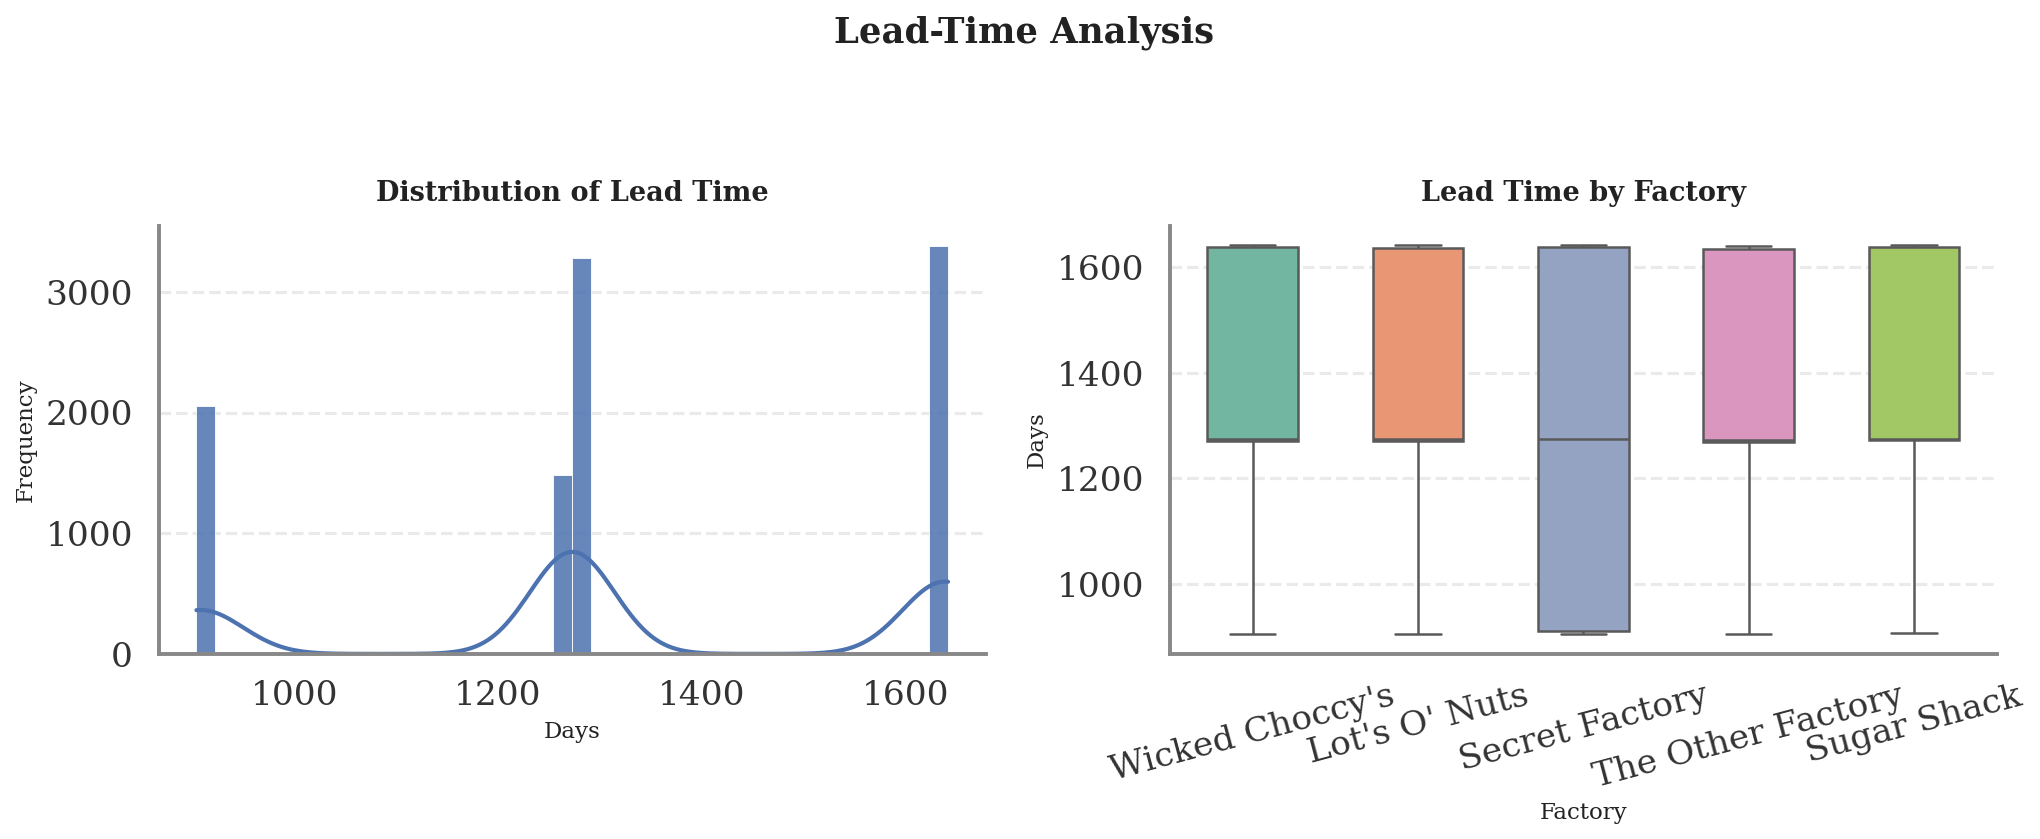
\includegraphics[width=\textwidth]{charts/hist_kde_box.png}
    \caption{Left: Lead time distribution showing a trimodal pattern
    corresponding to three order cohorts (early 2024, mid-2024, late 2025).
    Right: Lead time by factory --- four factories cluster in the upper range
    ($>$1,270 days); Secret Factory spans the full range (904--1,642 days).}
    \label{fig:lead_dist}
\end{figure}
% ------------------------------------------------

\subsection{Factory-Level Lead Time Patterns}

Box plot analysis of lead time segmented by factory reveals that
\fact{Lot's O' Nuts}, \fact{Wicked Choccy's}, \fact{Sugar Shack},
and \fact{The Other Factory} cluster predominantly in the upper
lead-time range (above 1,270 days), indicating that their order
activity is concentrated in earlier years.
\fact{Secret Factory}, by contrast, spans the full range
(904--1,642 days), suggesting its products --- Everlasting Gobstopper,
Wonka Gum, and Lickable Wallpaper --- were ordered uniformly across
all years with no temporal concentration or seasonal bias.
Lead time variability, measured as within-route standard deviation,
ranges from 210 to 311 days across factory-region combinations,
indicating substantial operational instability even on routes with
moderate average performance.

\subsection{Regional and Shipping Mode Analysis}

% ------------------------------------------------
\begin{figure}[H]
    \centering
    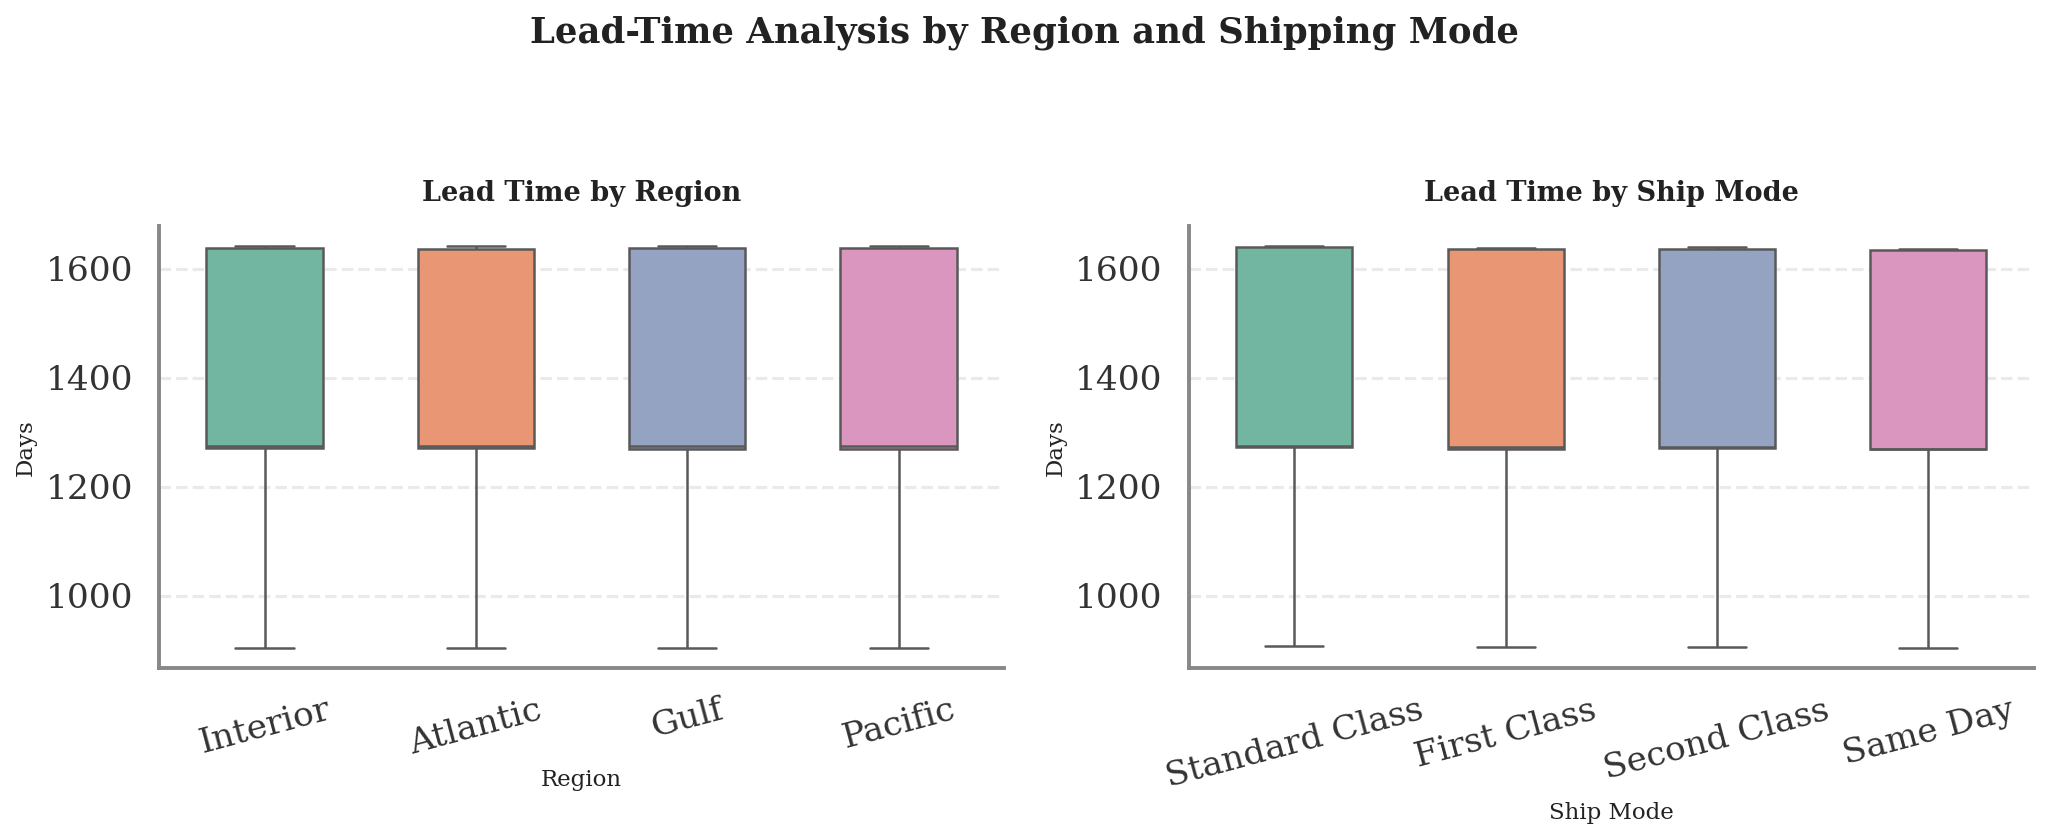
\includegraphics[width=\textwidth]{charts/boxnbox.png}
    \caption{Lead time distributions across all four regions
    (Atlantic, Gulf, Interior, Pacific) and all four ship modes
    (Standard Class, First Class, Second Class, Same Day) show
    nearly identical medians and interquartile ranges, confirming
    that lead time variation is systemic and temporal rather than
    route-specific.}
    \label{fig:region_shipmode}
\end{figure}
% ------------------------------------------------

Segmentation of lead times across all four \textbf{regions} and
all four \textbf{ship modes} reveals nearly identical medians and
interquartile ranges.
This uniformity confirms that lead time variation is
\textbf{systemic and temporal} rather than route-specific:
no particular region or shipping method produces meaningfully
faster or slower deliveries.
This is a critical operational finding --- it rules out
shipping-mode upgrades or regional prioritisation as effective
remediation strategies, and directs attention toward
factory-level reassignment as the primary lever for improvement.

\subsection{Financial Performance by Factory}

% ------------------------------------------------
\begin{figure}[H]
    \centering
    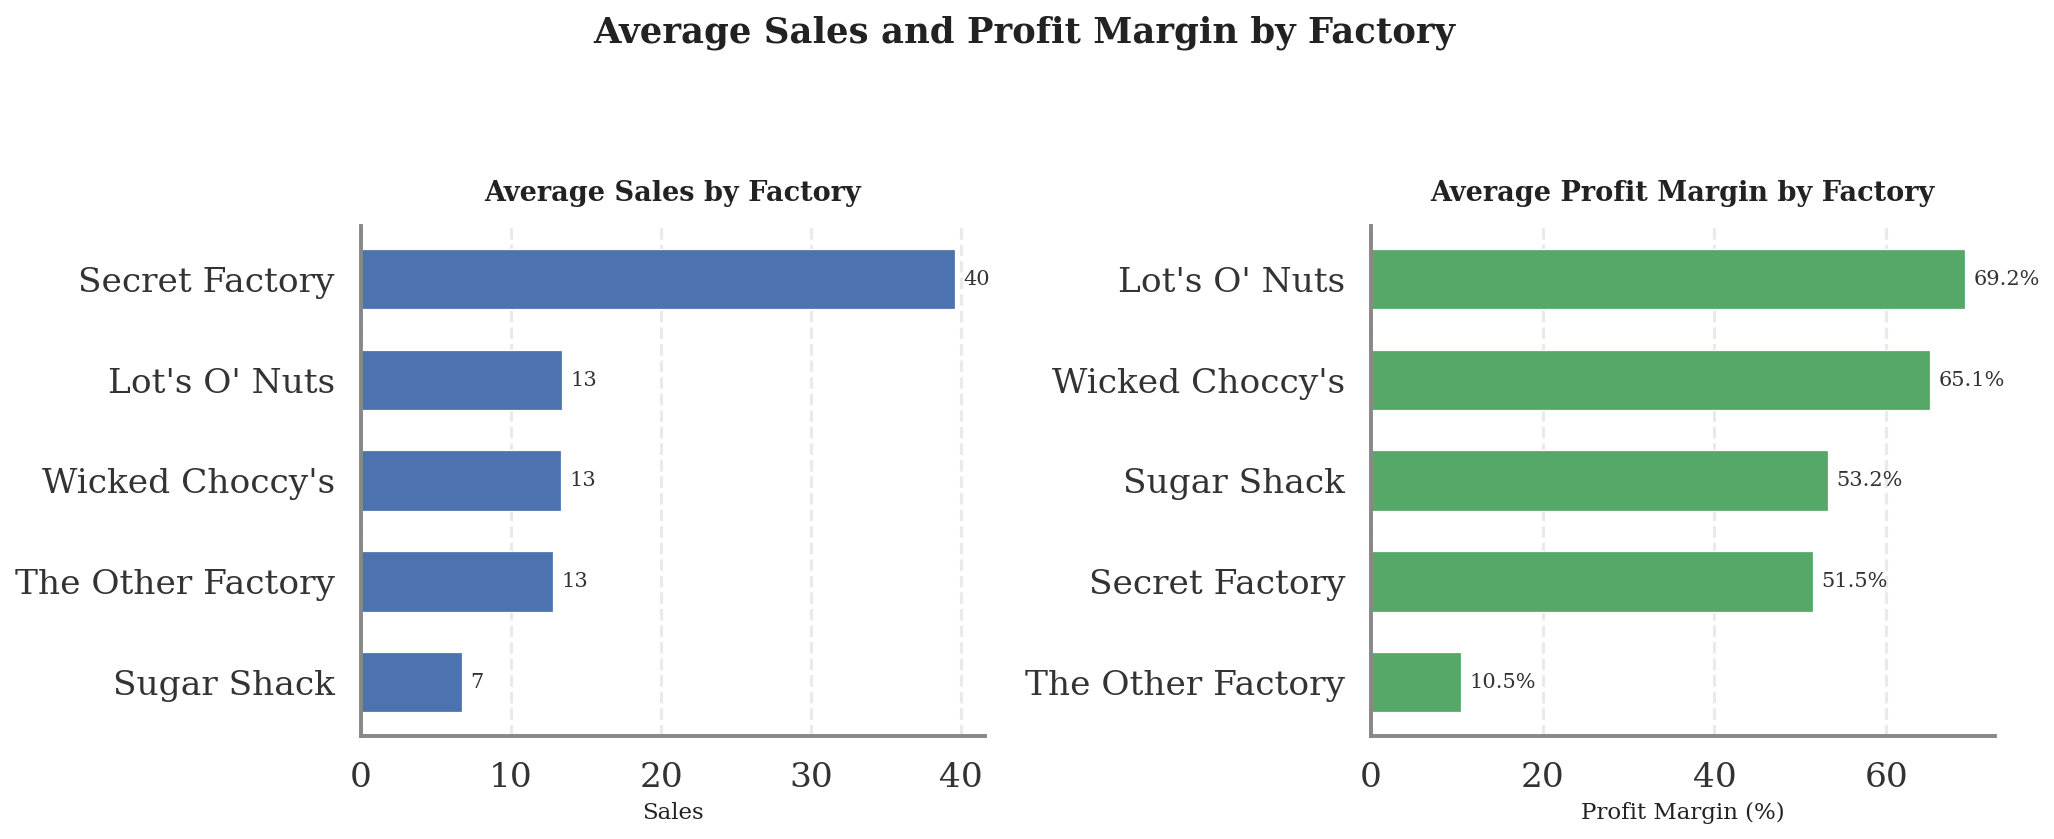
\includegraphics[width=\textwidth]{charts/avgsnp.png}
    \caption{Left: Secret Factory achieves the highest average
    revenue per order (\textasciitilde\$40) despite handling only
    217 orders. Right: Lot's O' Nuts and Wicked Choccy's lead on
    profit margin (\textasciitilde65--67\%); The Other Factory
    records a critically low weighted margin of \textasciitilde10\%,
    driven by Kazookles (7.7\% margin, 96 orders).}
    \label{fig:factory_financial}
\end{figure}
% ------------------------------------------------

Average sales analysis reveals \fact{Secret Factory} as the highest
revenue-generating factory (approximately \$40 per order) despite
handling only 217 orders, owing to its premium product portfolio.
\fact{Sugar Shack} recorded the lowest average sales, consistent
with its lower price-point sugar products.

Profit margin analysis uncovers a critical disparity:
\begin{itemize}[leftmargin=*]
    \item \textbf{Lot's O' Nuts} and \textbf{Wicked Choccy's}:
          approximately 65--67\% profit margin --- the most
          profitable factories in the network.
    \item \textbf{Sugar Shack}: approximately 52\%.
    \item \textbf{Secret Factory}: approximately 51\%.
    \item \textbf{The Other Factory}: approximately \textbf{10\%}
          --- a critically low weighted average driven almost entirely
          by Kazookles (7.7\% margin, 96 of 100 orders).
          Hair Toffee, its second product, carries a 77.8\% margin
          but represents only 4 orders, insufficient to offset the
          portfolio drag.
\end{itemize}

The Other Factory's low margin is a notable financial concern;
however, as Section~\ref{sec:clustering} and
Section~\ref{sec:recommendations} demonstrate, its
\emph{operational} performance --- consistent lead time efficiency
across all regions --- makes it the most strategically valuable
reassignment target in the network.

\subsection{Factory--Region Lead Time Heatmap}

Cross-tabulation of average lead time across all factory-region
combinations reveals notable route-level variation, after
accounting for the overall temporal effect on lead time.

% ------------------------------------------------
\begin{figure}[H]
    \centering
    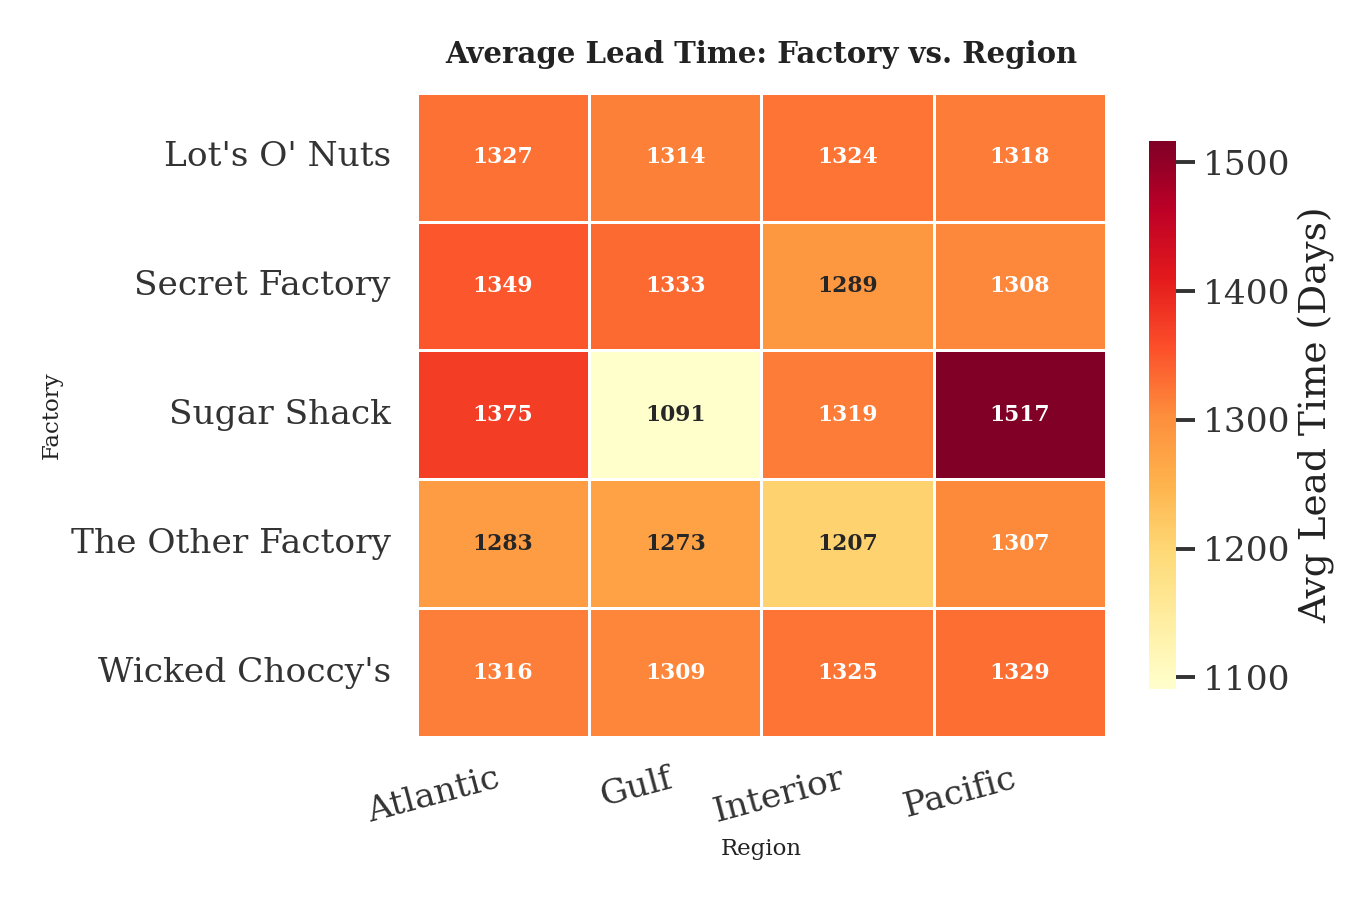
\includegraphics[width=\textwidth]{charts/heatmap1.png}
    \caption{Cross-tabulated average lead times (days) for each
    factory-region combination. Sugar Shack--Pacific (1,517 days)
    is the worst-performing route; Sugar Shack--Gulf (1,091 days)
    is the most efficient.}
    \label{fig:heatmap_lt}
\end{figure}
% ------------------------------------------------

\begin{table}[H]
\centering
\caption{Average Lead Time (Days) by Factory and Region}
\label{tab:lt_heatmap}
\renewcommand{\arraystretch}{1.15}
\begin{tabular}{lrrrr}
\toprule
\textbf{Factory} & \textbf{Atlantic} & \textbf{Gulf}
    & \textbf{Interior} & \textbf{Pacific} \\
\midrule
Lot's O' Nuts     & 1,327 & 1,314 & 1,324 & 1,318 \\
Secret Factory    & 1,349 & 1,333 & 1,289 & 1,308 \\
Sugar Shack       & 1,375 & \cellcolor{green!20}1,091
                          & 1,319 & \cellcolor{red!20}1,517 \\
The Other Factory & 1,283 & 1,273 & 1,207 & 1,307 \\
Wicked Choccy's   & 1,316 & 1,309 & 1,325 & 1,329 \\
\bottomrule
\end{tabular}
\end{table}

Key observations:
\begin{itemize}[leftmargin=*]
    \item \textbf{Sugar Shack--Pacific} (1,517 days): the
          worst-performing route, exceeding the network mean
          by 196 days --- nearly a 15\% penalty relative to
          the best-performing route.
    \item \textbf{Sugar Shack--Gulf} (1,091 days): anomalously
          fast despite a moderate shipping distance of
          approximately 1,321 miles, identifying Gulf-bound
          Sugar Shack fulfilment as an operational benchmark
          worth investigating.
    \item \textbf{The Other Factory} consistently posts
          below-average lead times across all four regions
          (1,207--1,307 days), confirming it as the most
          operationally efficient factory in the network.
\end{itemize}

\subsection{Correlation Analysis}

Pearson correlation analysis across the engineered numeric
features confirms two primary structural relationships
(Figure~\ref{fig:corr}).

% ------------------------------------------------
\begin{figure}[H]
    \centering
    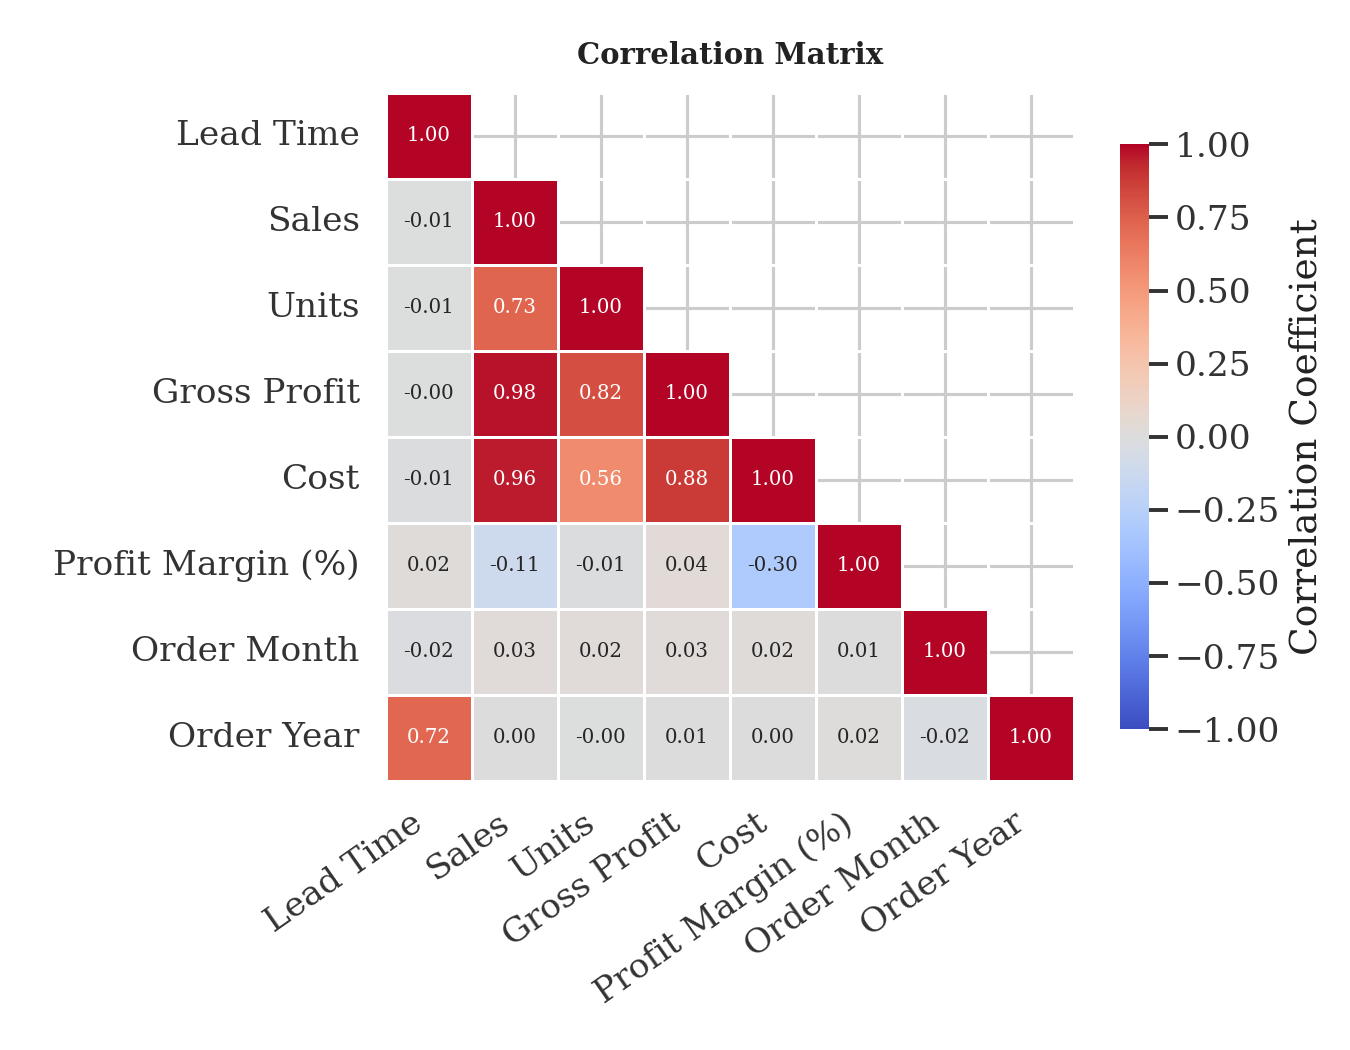
\includegraphics[width=\textwidth]{charts/correlation.png}
    \caption{Pearson correlation matrix. Order Year holds the
    strongest relationship with Lead Time ($r = 0.72$).
    Financial metrics (Sales, Gross Profit, Cost, Units) are
    highly inter-correlated ($r = 0.73$--$0.98$) as expected
    from their mathematical definitions.}
    \label{fig:corr}
\end{figure}
% ------------------------------------------------

\begin{itemize}[leftmargin=*]
    \item \textbf{Order Year $\leftrightarrow$ Lead Time}
          ($r = 0.72$): the strongest relationship in the dataset,
          confirming that the year of order placement is the
          primary driver of lead time variation --- consistent
          with the dataset's simulated forward-projection
          structure.
    \item \textbf{Financial inter-correlations}: Sales, Gross
          Profit, Cost, and Units are highly inter-correlated
          ($r = 0.73$--$0.98$), as expected given their
          mathematical relationships
          ($\text{Gross Profit} = \text{Sales} - \text{Cost}$).
    \item \textbf{All operational variables} --- Factory, Region,
          Ship Mode, Product, and Order Month --- show near-zero
          correlation with Lead Time ($|r| \leq 0.02$),
          indicating that routing decisions account for only a
          negligible share of lead time variance under the
          current static assignment structure. This motivates
          the use of clustering and scenario simulation
          (Sections~\ref{sec:clustering}--\ref{sec:recommendations})
          to surface the actionable operational signal that
          linear correlation cannot detect.
\end{itemize}

% ============================================================
\section{Key Insights}
\label{sec:insights}
% ============================================================

This section synthesises the most important findings from the
exploratory analysis into operationally relevant insights that
directly motivate the modelling and simulation work in subsequent
sections.

\subsection{Insight 1 --- The Network is Temporally Dominated}

Lead time variation in this dataset is driven overwhelmingly by
\textbf{when} an order was placed, not \textbf{how} it was routed.
Order Year has a Pearson correlation of $r = 0.72$ with Lead Time,
implying it individually accounts for approximately 52\% of lead
time variance ($r^2 \approx 0.518$).
The full nine-feature predictive model explains 53\% of variance
($R^2 = 0.53$), indicating that the eight remaining features
contribute only marginally beyond Order Year alone.
Factory identity contributes essentially zero independent predictive
power. This means that headline lead-time comparisons across factories
or regions will be confounded by order-cohort composition and must
be interpreted with caution.

\subsection{Insight 2 --- Factory Capacity is Critically Imbalanced}

Two factories --- Lot's O' Nuts and Wicked Choccy's --- absorb
\textbf{96.5\%} of all orders (9,844 out of 10,194), while
serving all four regions simultaneously.
The Other Factory, which demonstrates the best lead-time performance
network-wide, handles only \textbf{100 orders} (1.0\% of volume)
and is operating far below its potential capacity.
This structural imbalance is the single most important operational
finding in the dataset and the primary target of the
reassignment recommendations in Section~\ref{sec:recommendations}.

\subsection{Insight 3 --- The Other Factory is the Operational Benchmark}

Across every factory-region combination, The Other Factory
consistently records the shortest average lead times:
Atlantic (1,283 days), Gulf (1,273 days), Interior (1,207 days),
and Pacific (1,307 days).
Its overall average lead time of \fact{1,267.3 days} is the lowest
of any factory in the network --- approximately 53 days faster than
Lot's O' Nuts and 57 days faster than Wicked Choccy's on a
network-wide basis.

\subsection{Insight 4 --- Lot's O' Nuts and Wicked Choccy's are Congested}

Route clustering (Section~\ref{sec:clustering}) classifies all
routes served by Lot's O' Nuts and Wicked Choccy's as
\emph{Congested Routes} --- the second-worst operational category.
These two factories handle 9,844 orders, creating systemic
throughput pressure that affects all four regions uniformly.
Critically, the congestion is a \textbf{volume problem, not a
geographic one}: lead times are uniformly elevated regardless
of region or ship mode, ruling out targeted route adjustments
as a fix.

\subsection{Insight 5 --- Secret Factory is Mid-Range; Sugar Shack is Inconsistent}

Secret Factory routes are classified as \emph{Moderate Routes} ---
mid-range lead times across all regions with low order volume
(217 orders). Its operational profile is stable but unremarkable.

Sugar Shack exhibits the highest route-level inconsistency in the
network: its Gulf route is classified as \emph{Optimised}
(1,091 days --- the best single route in the dataset), while its
Atlantic, Interior, and Pacific routes are classified as
\emph{Bottleneck Routes}. Sugar Shack--Pacific, at 1,517 days,
is the worst-performing individual route in the entire network ---
a 426-day gap relative to its own Gulf route.

\subsection{Insight 6 --- The Other Factory's Low Margin is a Financial Risk, Not an Operational One}

The Other Factory's weighted profit margin of approximately 10\%
--- driven by Kazookles (7.7\% margin, 96 of 100 orders) --- is a
financial concern but does not affect its operational efficiency
as a fulfilment centre.
Simulation results confirm that reassigning other products
\emph{to} The Other Factory does not degrade their profit margins
(impact $< 0.05\%$).
The financial concern is specific to The Other Factory's existing
product line and warrants a separate pricing or product-mix review
outside the scope of this analysis.

\subsection{Insight 7 --- Hair Toffee Cannot Be Reassigned}

Hair Toffee records the highest average lead time of any product
in the dataset (approximately 1,455 days) and falls into the
\emph{Slow \& Risky} product cluster.
However, it is \emph{already manufactured at The Other Factory} ---
the fastest factory in the network.
Its elevated lead time therefore cannot be resolved through factory
reassignment; it likely reflects a geographic mismatch between the
factory's location and Hair Toffee's demand centres, or
product-specific operational constraints at The Other Factory.
Hair Toffee is accordingly \textbf{excluded from the reassignment
simulation} and requires a separate operational investigation.

\subsection{Insight 8 --- Everlasting Gobstopper is the Highest-Priority Reassignment Candidate}

Everlasting Gobstopper (currently at Secret Factory) records an
average lead time of 1,394.7 days combined with an 80\% profit
margin --- the highest margin in the dataset.
This combination of extreme operational inefficiency and high
profitability places it at \textbf{rank \#1} in the composite
priority scoring framework.
It should be noted that this product has only 3 recorded orders
in the dataset, which limits the statistical reliability of its
average lead time estimate. The ranking reflects the scoring
framework's output and should be treated as directionally
informative rather than conclusive pending higher order volumes.

% ============================================================
\section{Predictive Modelling}
\label{sec:model}
% ============================================================

\subsection{Objective and Feature Matrix}

The predictive modelling objective is to estimate order lead time
from observable features available at the time of order.
This serves two purposes: (1) to quantify how much of lead time
variation is explainable by the available features; and (2) to
identify which features carry the most predictive signal,
informing the design of the scenario simulation engine.

The final feature matrix $\mathbf{X}$ contains 9 variables:

\begin{itemize}[leftmargin=*]
    \item \textbf{Categorical (label-encoded):} Product Encoded,
          Factory Encoded, Region Encoded, Ship Mode Encoded.
    \item \textbf{Temporal:} Order Month, Order Year.
    \item \textbf{Financial (Min-Max normalised):} Sales, Units,
          Profit Margin (\%).
\end{itemize}

The target variable $y$ is Lead Time (days).
The dataset was split 80/20 into training (8,155 rows) and test
(2,039 rows) sets using \texttt{random\_state=42} for
reproducibility.

\subsection{Models Trained}

Three regression models were evaluated:

\begin{enumerate}[leftmargin=*, label=\arabic*.]
    \item \textbf{Linear Regression} --- baseline model with
          interpretable coefficients.
    \item \textbf{Random Forest Regressor} \citep{breiman2001} ---
          ensemble of 100 decision trees (\texttt{random\_state=42}).
    \item \textbf{Gradient Boosting Regressor} \citep{friedman2001} ---
          sequential boosting with 100 estimators (\texttt{random\_state=42}).
\end{enumerate}

\subsection{Model Performance}

\begin{table}[H]
\centering
\caption{Predictive Model Comparison (Test Set, n = 2,039)}
\label{tab:model_comparison}
\renewcommand{\arraystretch}{1.2}
\begin{tabular}{lrrr}
\toprule
\textbf{Model} & \textbf{RMSE (days)} & \textbf{MAE (days)}
    & $\mathbf{R^2}$ \\
\midrule
\rowcolor{lightgray}
Linear Regression   & \textbf{182.16} & 181.21 & \textbf{0.5308} \\
Gradient Boosting   & 182.70 & 180.99 & 0.5280 \\
Random Forest       & 203.86 & 180.28 & 0.4124 \\
\bottomrule
\end{tabular}
\end{table}

\textbf{Linear Regression} achieves the best overall performance
with the lowest RMSE (182.16 days) and highest $R^2$ (0.5308),
and was selected as the model for downstream lead time estimation.
The moderate $R^2$ of 0.53 indicates that approximately
\textbf{53\% of lead time variability} is explained by the
selected features, consistent with the correlation analysis
confirming Order Year as the dominant driver.

Random Forest, despite being an ensemble method, underperforms
both simpler models on RMSE and $R^2$. This is consistent with
the dataset's predominantly linear temporal structure: ensemble
tree methods gain their advantage from capturing complex
non-linear interactions, which are largely absent here given
that a single temporal feature dominates the signal.

% ------------------------------------------------
\begin{figure}[H]
    \centering
    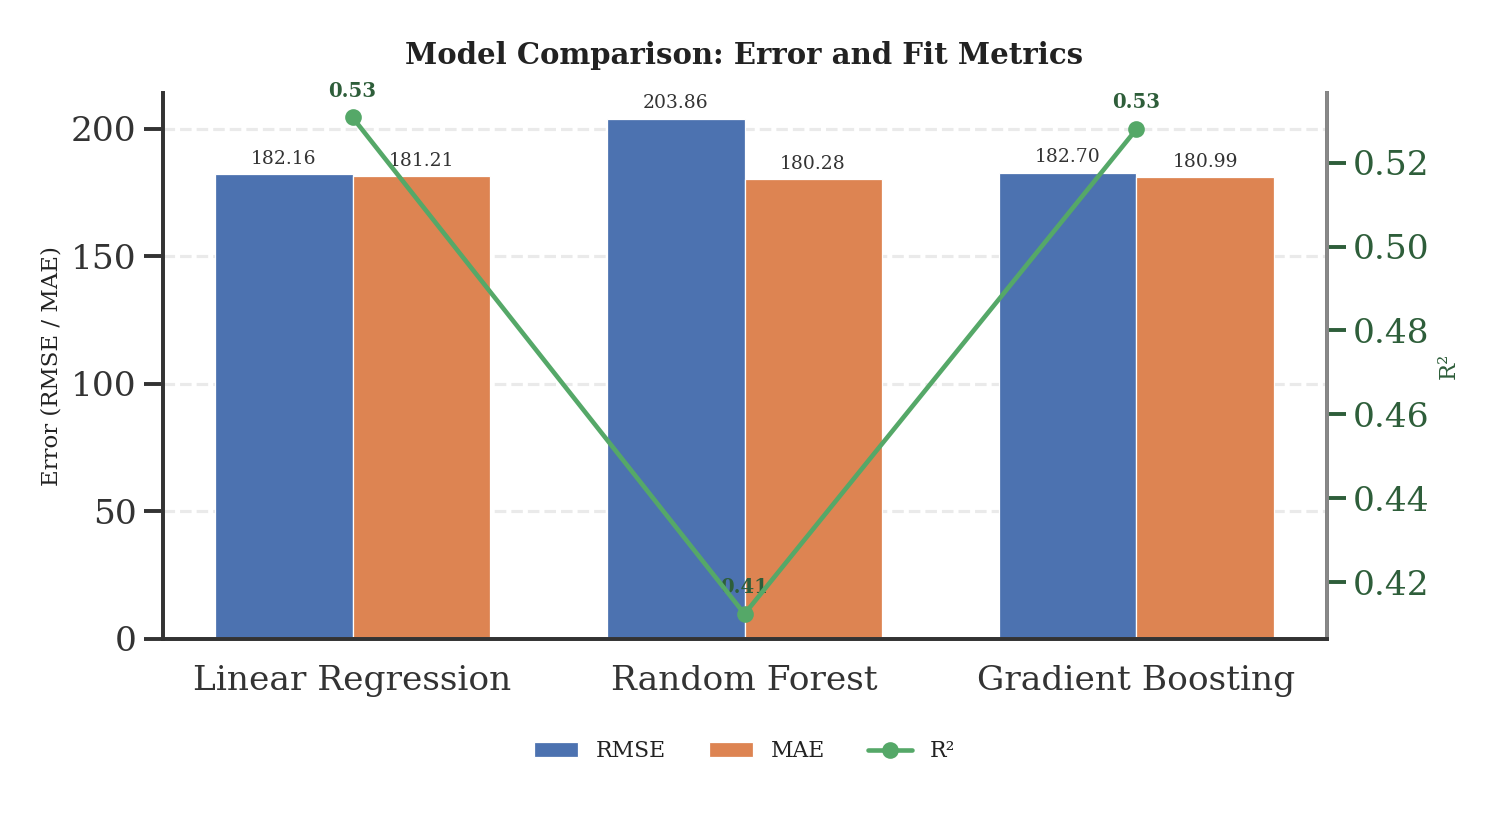
\includegraphics[width=\textwidth]{charts/compare.png}
    \caption{Visual comparison of RMSE, MAE, and $R^2$ across
    the three regression models. Linear Regression achieves the
    best RMSE and $R^2$; all three models produce similar MAE,
    reflecting the dominant role of Order Year across all
    modelling approaches.}
    \label{fig:model_comparison}
\end{figure}
% ------------------------------------------------

\subsection{Feature Importance}

Table~\ref{tab:lr_coef} presents feature importance from both
models. Linear Regression coefficients reflect the magnitude
and direction of each feature's marginal effect on predicted
lead time (in days, on the original scale). Gradient Boosting
importances reflect the relative contribution of each feature
to split-based variance reduction across all trees; these are
unitless and sum to 1.0.

\begin{table}[H]
\centering
\caption{Feature Importance: Linear Regression Coefficients
and Gradient Boosting Importances (Sorted by Absolute
LR Coefficient)}
\label{tab:lr_coef}
\renewcommand{\arraystretch}{1.12}
\begin{tabular}{lrr}
\toprule
\textbf{Feature} & \textbf{LR Coefficient}
    & \textbf{GB Importance} \\
\midrule
Order Year         &  381.874 & 0.9707 \\
Profit Margin (\%) &   20.194 & 0.0012 \\
Units              &  -15.773 & 0.0014 \\
Sales              &   -8.466 & 0.0067 \\
Ship Mode Encoded  &   -2.266 & 0.0026 \\
Product Encoded    &    1.054 & 0.0018 \\
Factory Encoded    &    0.908 & 0.0000 \\
Region Encoded     &   -0.369 & 0.0073 \\
Order Month        &   -0.130 & 0.0082 \\
\bottomrule
\end{tabular}
\end{table}

Both methods converge on the same conclusion: \textbf{Order Year}
dominates with a Linear Regression coefficient of 381.87 ---
approximately 19$\times$ larger than the next most influential
feature --- and a Gradient Boosting importance of 0.9707,
attributing \textbf{97.07\% of predictive power} to a single
feature. Factory Encoded records \textbf{zero importance} in
the Gradient Boosting model, confirming that factory identity
carries no detectable non-linear signal beyond what is already
captured by temporal features.

This result is not a modelling failure --- it is a structural
finding. The dataset's static assignment rules mean that each
factory always serves the same products to the same regions,
making factory and temporal effects nearly collinear. Unlocking
the operational signal embedded in factory-level differences
requires the simulation framework described in
Section~\ref{sec:recommendations}, which isolates factory
effects by holding temporal variables constant across
reassignment scenarios.

% ============================================================
\section{Route and Product Clustering}
\label{sec:clustering}
% ============================================================

\subsection{Route Clustering --- Motivation}

Because the predictive model confirms that factory identity
contributes negligible predictive power to lead time in
isolation, a complementary clustering approach is used to
surface the \emph{relative} performance differences across
factory-region routes. Rather than predicting absolute lead
time, clustering groups routes by their combined operational
and financial profile, enabling categorical classification of
network performance.

\subsection{Feature Selection and Scaling}

Eight features were used for route clustering, standardised
independently using \texttt{StandardScaler} to ensure
zero-mean, unit-variance scaling across heterogeneous units:

\begin{itemize}[leftmargin=*, itemsep=0pt]
    \item \textit{Avg Lead Time}, \textit{Lead Time Std Dev}
          (within-route variability), \textit{Order Count}
    \item \textit{Avg Sales}, \textit{Avg Profit Margin},
          \textit{Avg Cost}
    \item \textit{Shipping Distance} (Haversine, miles)
    \item \textit{Factory Utilisation} (\% of total network
          orders)
\end{itemize}

The inclusion of Lead Time Std Dev captures route instability
beyond what average lead time alone reveals --- two routes with
identical means but different variances carry different
operational risk profiles.

\subsection{Optimal K Selection}

The elbow method and silhouette scoring \citep{rousseeuw1987}
were applied over $K \in \{2, \ldots, 7\}$. Silhouette scores
are reported in Table~\ref{tab:silhouette}.

\begin{table}[H]
\centering
\caption{Silhouette Scores for Route Clustering
         by Number of Clusters}
\label{tab:silhouette}
\renewcommand{\arraystretch}{1.12}
\begin{tabular}{cc}
\toprule
\textbf{K} & \textbf{Silhouette Score} \\
\midrule
2 & 0.3170 \\
3 & 0.3766 \\
4 & 0.3947 \\
\rowcolor{lightgray}
5 & \textbf{0.4119} \\
6 & 0.4080 \\
7 & 0.3892 \\
\bottomrule
\end{tabular}
\end{table}

$K = 5$ yields the highest silhouette score (0.4119) and was
selected as the optimal number of route clusters.

\subsection{Cluster Profiles and Labels}

The five clusters were labelled by ascending average lead time
as: \emph{Optimised Routes}, \emph{Efficient Routes},
\emph{Moderate Routes}, \emph{Congested Routes}, and
\emph{Bottleneck Routes}. Cluster profiles are summarised in
Table~\ref{tab:cluster_profiles}.

\begin{table}[H]
\centering
\caption{Route Cluster Profiles (K = 5)}
\label{tab:cluster_profiles}
\renewcommand{\arraystretch}{1.15}
\begin{tabular}{lrrrrr}
\toprule
\textbf{Label} & \textbf{Avg Lead} & \textbf{Avg Std}
    & \textbf{Avg Distance} & \textbf{Avg Util.}
    & \textbf{Total Orders} \\
 & \textbf{Time (days)} & \textbf{Dev (days)}
    & \textbf{(miles)} & \textbf{(\%)} & \\
\midrule
Optimised Routes  & 1,091.2 & 210.4 & 1,321.4 &  0.3 &     4 \\
Efficient Routes  & 1,267.3 & 265.2 &   888.1 &  1.0 &   100 \\
Moderate Routes   & 1,319.7 & 293.2 &   933.5 &  2.1 &   217 \\
Congested Routes  & 1,320.2 & 261.9 & 1,155.8 & 48.3 & 9,844 \\
Bottleneck Routes & 1,403.6 & 240.0 & 1,057.1 &  0.3 &    29 \\
\bottomrule
\end{tabular}
\end{table}

Figure~\ref{fig:route_heatmap} shows the route label
assignment for every factory-region pair, and
Figure~\ref{fig:route_bubble} plots each route by
shipping distance and average lead time, with bubble
size proportional to order volume.

% ------------------------------------------------
\begin{figure}[H]
    \centering
    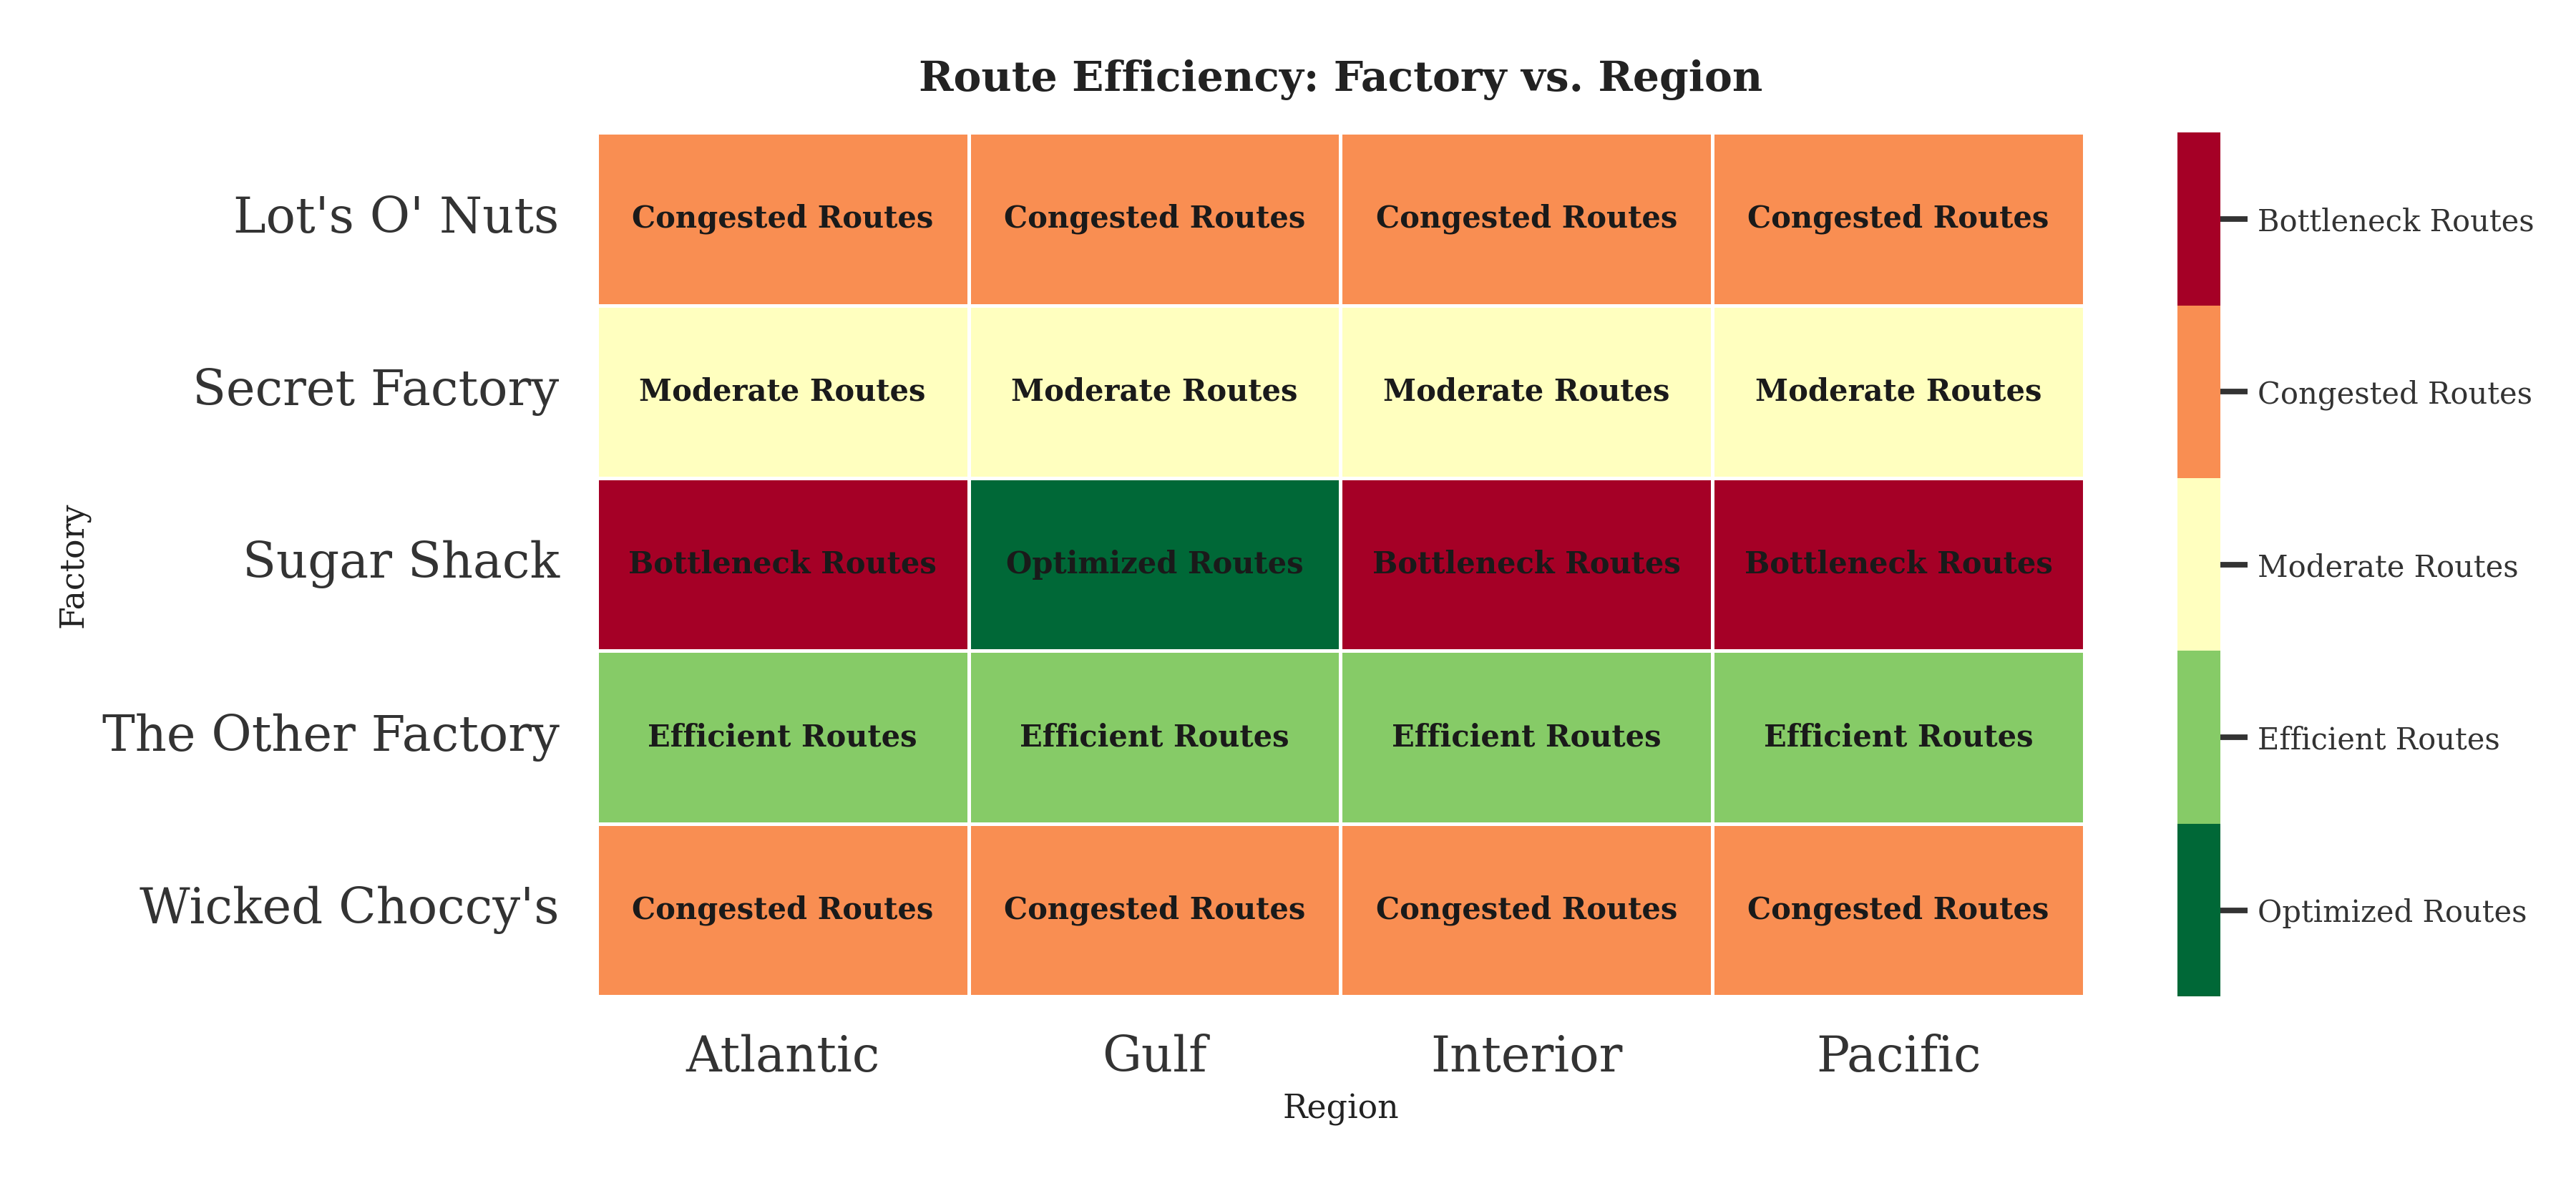
\includegraphics[width=\textwidth]{charts/heatmap2.png}
    \caption{Route classification heatmap. Lot's O' Nuts
    and Wicked Choccy's are Congested across all regions;
    The Other Factory is Efficient across all regions;
    Secret Factory is Moderate across all regions; Sugar
    Shack is highly inconsistent --- Optimised in Gulf,
    Bottleneck in Atlantic, Interior, and Pacific.}
    \label{fig:route_heatmap}
\end{figure}
% ------------------------------------------------

% ------------------------------------------------
\begin{figure}[H]
    \centering
    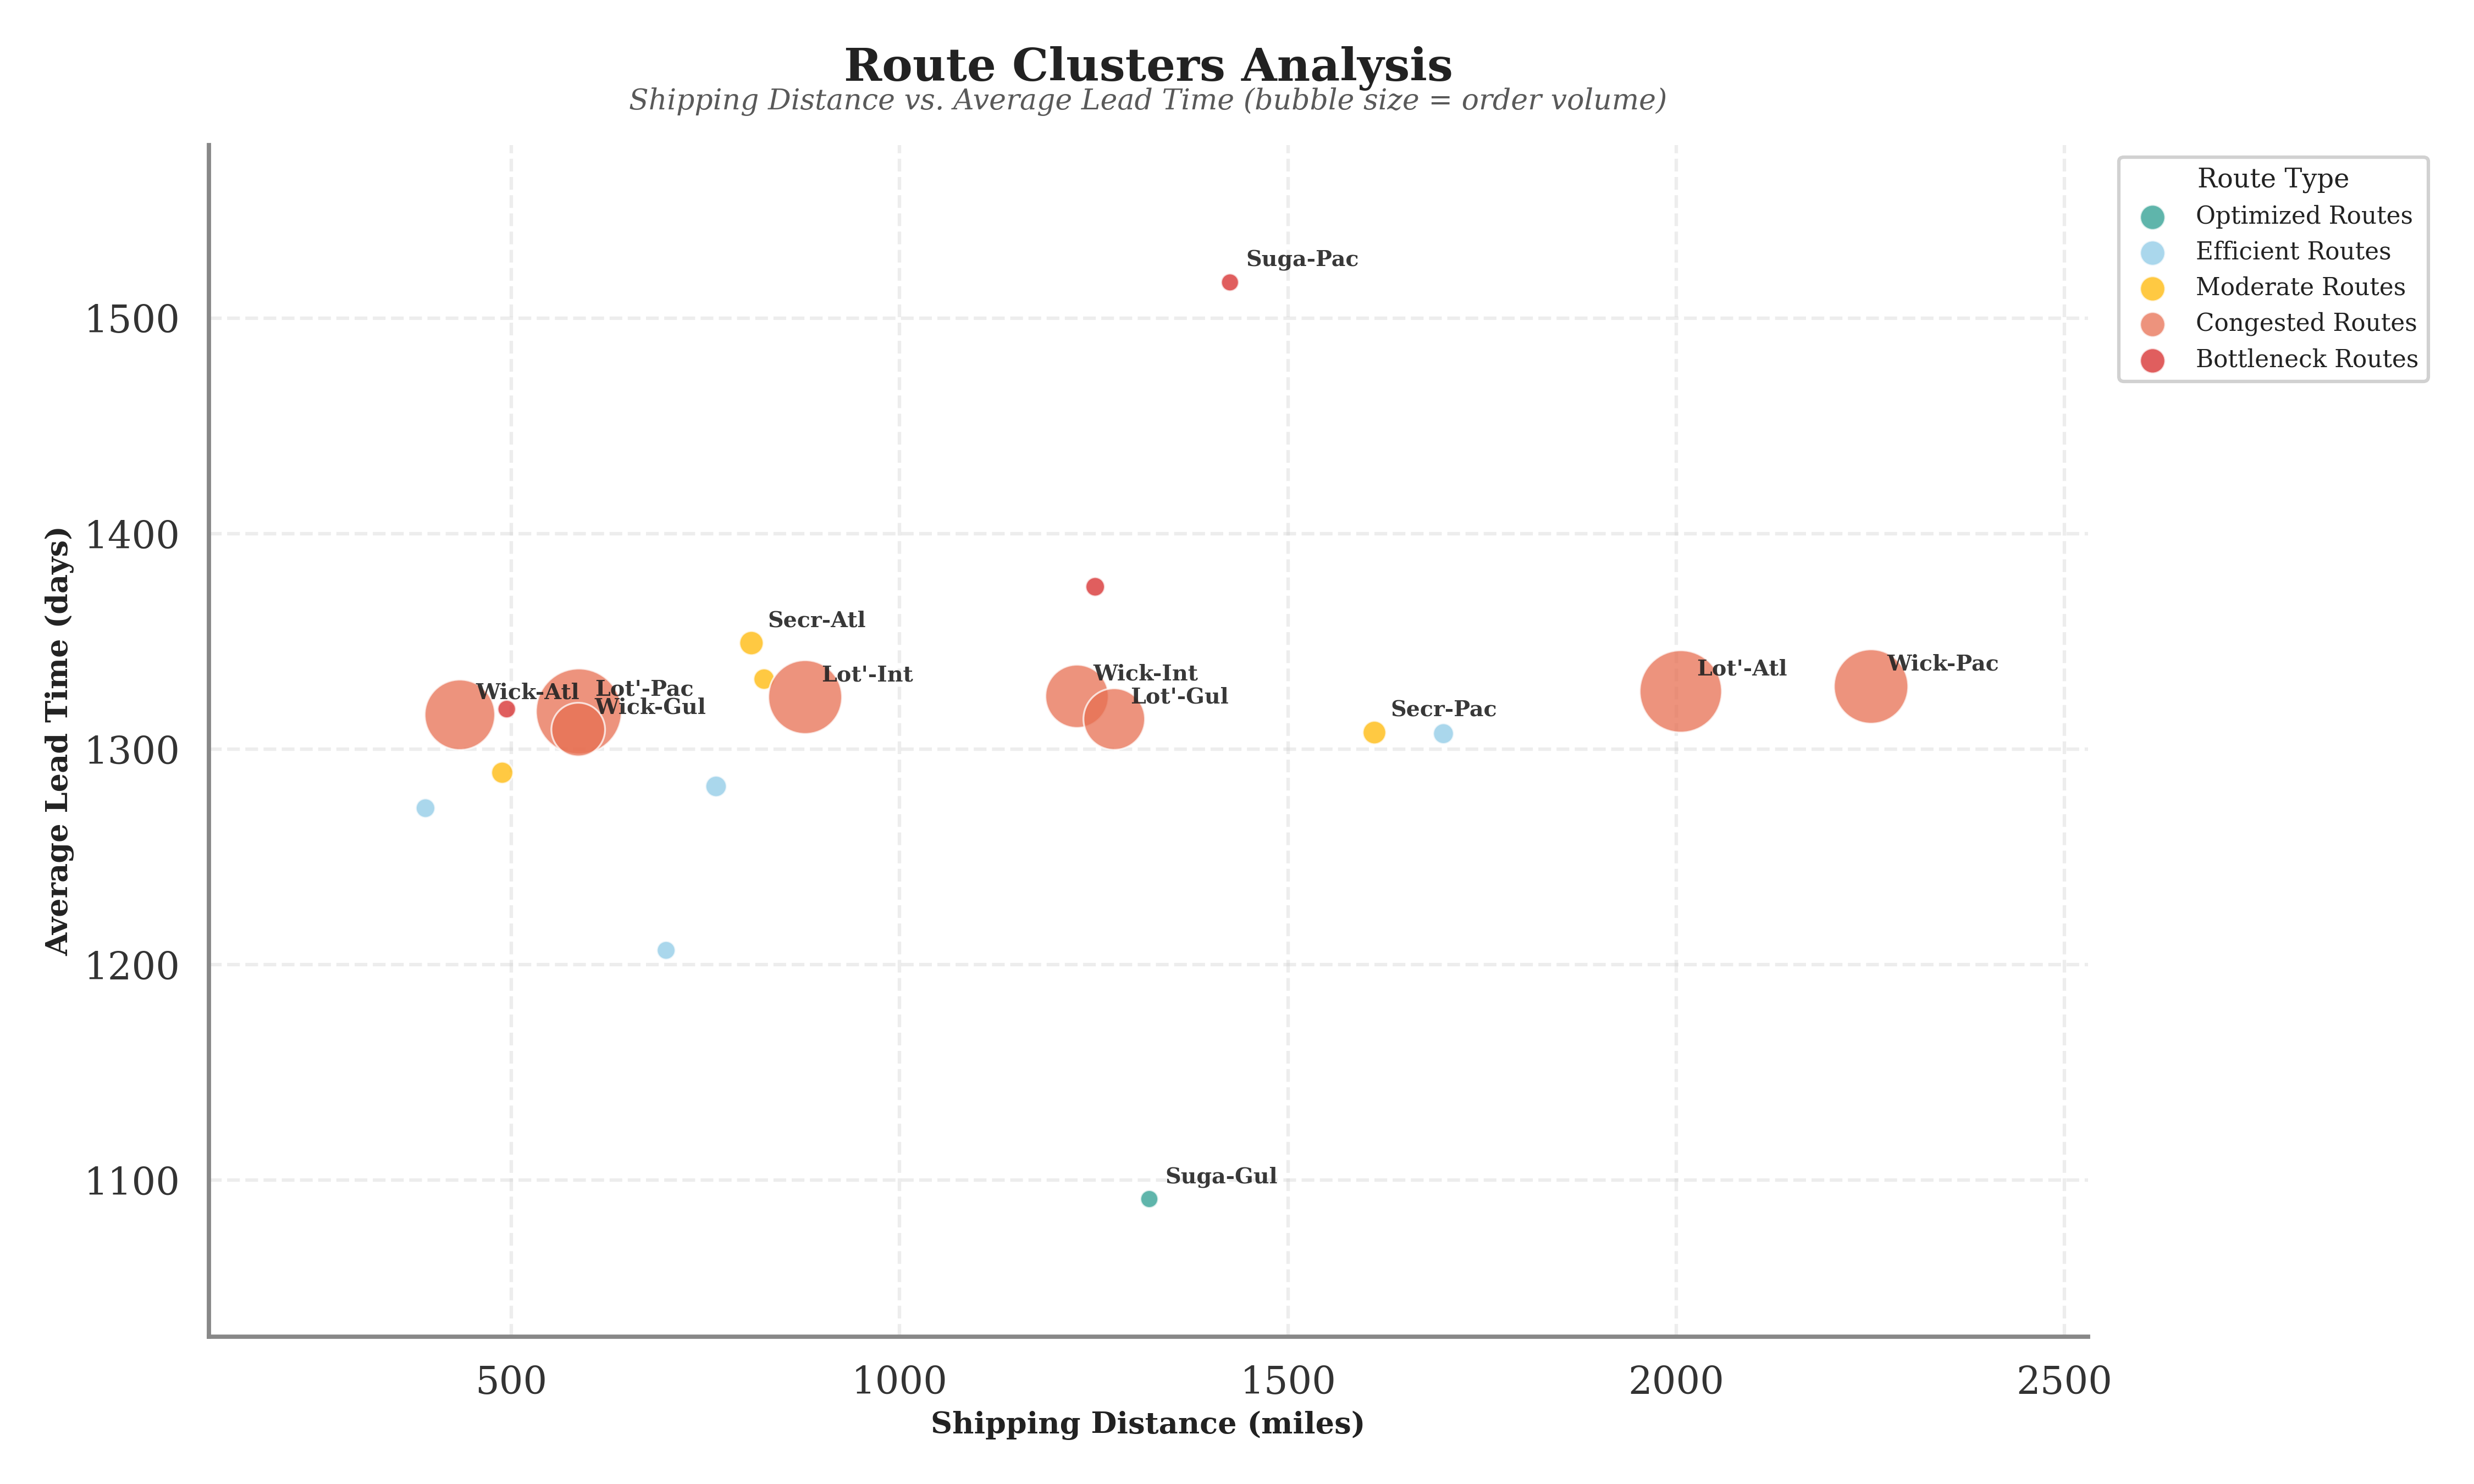
\includegraphics[width=\textwidth]{charts/routeCluster.png}
    \caption{Route cluster bubble chart. Sugar Shack--Pacific
    sits in the upper portion (highest lead time despite
    moderate distance). Sugar Shack--Gulf is an anomalous
    low outlier (fast despite 1,321 miles). Congested
    routes (Lot's O' Nuts and Wicked Choccy's, large
    bubbles) cluster around 1,310--1,330 days regardless
    of distance, confirming that their elevated lead times
    are volume-driven rather than geography-driven.}
    \label{fig:route_bubble}
\end{figure}
% ------------------------------------------------

The heatmap reveals a clean factory-level pattern: each
factory receives a \emph{uniform} classification across
all four regions, with the sole exception of Sugar Shack.
This confirms that route performance is primarily determined
by factory-level characteristics --- most notably order volume
and utilisation --- rather than the destination region.

\subsection{Product Clustering}

A separate K-Means clustering \citep{macqueen1967} was applied
at the product level using four features: \textit{Avg Lead Time},
\textit{Lead Time Std Dev}, \textit{Avg Profit Margin},
and \textit{Avg Sales}. Silhouette scores across
$K \in \{2, \ldots, 6\}$ are reported in
Table~\ref{tab:prod_silhouette}; $K = 3$ was selected.

\begin{table}[H]
\centering
\caption{Silhouette Scores for Product Clustering}
\label{tab:prod_silhouette}
\renewcommand{\arraystretch}{1.12}
\begin{tabular}{cc}
\toprule
\textbf{K} & \textbf{Silhouette Score} \\
\midrule
2 & 0.3619 \\
\rowcolor{lightgray}
3 & \textbf{0.3861} \\
4 & 0.3359 \\
5 & 0.3661 \\
6 & 0.3174 \\
\bottomrule
\end{tabular}
\end{table}

The three product clusters are labelled by ascending average
lead time as \emph{Fast \& Profitable},
\emph{Average Performer}, and \emph{Slow \& Risky}.
Products in each cluster are:

\begin{itemize}[leftmargin=*]
    \item \textbf{Fast \& Profitable:} Fun Dip, Kazookles
          --- lowest average lead times in the dataset.
          Note that Kazookles carries only a 7.7\% profit
          margin, making it fast but financially weak.
    \item \textbf{Average Performer:} Wonka Gum, Fizzy
          Lifting Drinks, Nerds, and all five Chocolate
          division Wonka Bars --- moderate lead times,
          high order volumes, and solid margins
          (64--71\%). These represent the core of the
          distribution network and are the primary
          candidates for reassignment due to their
          high volume impact.
    \item \textbf{Slow \& Risky:} Everlasting Gobstopper,
          Hair Toffee, Lickable Wallpaper --- highest lead
          times and the greatest operational urgency.
          Everlasting Gobstopper is the highest-priority
          reassignment candidate (80\% margin, 1,394.7
          days). Lickable Wallpaper represents moderate
          risk (50\% margin, 1,339 days).
\end{itemize}

\textbf{Note on Hair Toffee:} Hair Toffee records the
highest average lead time in the dataset
(approximately 1,455 days). However, it is already
manufactured at The Other Factory --- the most efficient
factory in the network. Its elevated lead time cannot
therefore be remedied by factory reassignment and likely
reflects structural constraints specific to this product.
Hair Toffee is excluded from the reassignment simulation
and flagged for separate operational investigation.

% ============================================================
\section{Factory Reassignment Recommendations}
\label{sec:recommendations}
% ============================================================

\subsection{Simulation Framework}

The simulation engine evaluates all feasible factory
reassignment scenarios for each product. For a given product
currently manufactured at factory $f_0$, the simulation tests
reassignment to every alternative factory
$f_i \in \mathcal{F} \setminus \{f_0\}$. Each scenario
estimates:

\begin{align}
    \hat{L}_{f_i} &= \bar{L}_{f_i} +
        (\bar{L}_{f_0,p} - \bar{L}_{f_0})
        \label{eq:pred_lt} \\
    \Delta L &= \bar{L}_{f_0,p} - \hat{L}_{f_i}
        \label{eq:reduction} \\
    \Delta L_{\%} &= \frac{\Delta L}{\bar{L}_{f_0,p}}
        \times 100
        \label{eq:pct} \\
    D_{\text{saved}} &= \Delta L \times n_p
        \label{eq:days_saved}
\end{align}

where $\bar{L}_{f_i}$ is the network-wide average lead time
for factory $f_i$, $\bar{L}_{f_0,p}$ is the current
product-level average lead time, $\bar{L}_{f_0}$ is the
current factory average, and $n_p$ is the product order count.
Only scenarios with $\Delta L > 0$ are retained.
The composite priority score is as defined in
Equation~\ref{eq:score} (Section~\ref{sec:data}), weighting
60\% lead time reduction, 30\% predicted margin, and 10\%
normalised order volume. The top-scoring reassignment per
product is retained as the final recommendation.

\subsection{Final Recommendations}

\begin{table}[H]
\centering
\caption{Final Factory Reassignment Recommendations
         (All 13 Products, Sorted by Priority Score)}
\label{tab:final_recommendations}
\renewcommand{\arraystretch}{1.15}
\small
\begin{tabularx}{\textwidth}{rp{4.5cm}p{2.8cm}p{2.8cm}rr}
\toprule
\textbf{Rank} & \textbf{Product} & \textbf{Current Factory}
    & \textbf{Rec. Factory}
    & \textbf{Save (days)} & \textbf{Score} \\
\midrule
1  & Everlasting Gobstopper            & Secret Factory
    & The Other Factory & 52 & 26.1 \\
2  & Fizzy Lifting Drinks              & Sugar Shack
    & The Other Factory & 58 & 25.3 \\
3  & Wonka Bar -- Nutty Crunch Surprise & Lot's O' Nuts
    & The Other Factory & 53 & 25.1 \\
4  & Wonka Bar -- Scrumdiddlyumptious  & Lot's O' Nuts
    & The Other Factory & 53 & 25.0 \\
5  & Wonka Bar -- Fudge Mallows        & Lot's O' Nuts
    & The Other Factory & 53 & 24.9 \\
6  & Laffy Taffy                       & Sugar Shack
    & The Other Factory & 58 & 24.1 \\
7  & Wonka Bar -- Triple Dazzle Caramel & Wicked Choccy's
    & The Other Factory & 52 & 24.0 \\
8  & Wonka Bar -- Milk Chocolate       & Wicked Choccy's
    & The Other Factory & 52 & 23.0 \\
9  & Lickable Wallpaper                & Secret Factory
    & The Other Factory & 52 & 22.8 \\
10 & Wonka Gum                         & Secret Factory
    & The Other Factory & 52 & 22.5 \\
11 & SweeTARTS                         & Sugar Shack
    & The Other Factory & 58 & 22.4 \\
12 & Nerds                             & Sugar Shack
    & The Other Factory & 58 & 22.1 \\
13 & Fun Dip                           & Sugar Shack
    & The Other Factory & 58 & 21.9 \\
\midrule
\multicolumn{4}{r}{\textbf{Total Estimated Days Saved}}
    & \textbf{534,218} & \\
\multicolumn{4}{r}{\textbf{Average Reduction per Product}}
    & \textbf{54.8 days} & \\
\bottomrule
\end{tabularx}
\end{table}

The overwhelming finding is unambiguous: \textbf{The Other
Factory is the universally optimal reassignment destination}
for all 13 products. This outcome is a direct structural
consequence of The Other Factory being both the fastest
factory in the network (average lead time: 1,267.3 days)
and the most underutilised (1.0\% of total order volume).
The convergence of every recommendation on a single factory
underscores the severity of the current capacity imbalance
and the magnitude of the available operational improvement.

\subsection{Risk and Margin Safety Panel}

Risk was assessed based on each product's predicted
post-reassignment profit margin, categorised as:

\begin{itemize}[leftmargin=*, itemsep=2pt]
    \item \textcolor{riskhigh}{\textbf{HIGH RISK:}}
          Predicted margin $<$ 20\%
    \item \textcolor{riskmod}{\textbf{MODERATE RISK:}}
          Predicted margin 20--50\%
    \item \textcolor{risklow}{\textbf{LOW RISK:}}
          Predicted margin $>$ 50\%
\end{itemize}

\begin{table}[H]
\centering
\caption{Risk and Margin Safety Assessment (Post-Reassignment)}
\label{tab:risk}
\renewcommand{\arraystretch}{1.2}
\begin{tabular}{llrrr}
\toprule
\textbf{Risk} & \textbf{Product}
    & \textbf{Current} & \textbf{Predicted}
    & \textbf{Days} \\
 & & \textbf{Margin (\%)} & \textbf{Margin (\%)}
    & \textbf{Saved} \\
\midrule
\rowcolor{risklowbg} \textcolor{risklow}{LOW} & Everlasting Gobstopper           & 80.0 & 80.0 & 52 \\
\rowcolor{risklowbg} \textcolor{risklow}{LOW} & Fizzy Lifting Drinks             & 60.0 & 60.0 & 58 \\
\rowcolor{riskmodbg} \textcolor{riskmod}{MOD} & Fun Dip                          & 40.0 & 40.0 & 58 \\
\rowcolor{risklowbg} \textcolor{risklow}{LOW} & Laffy Taffy                      & 62.3 & 62.3 & 58 \\
\rowcolor{risklowbg} \textcolor{risklow}{LOW} & Lickable Wallpaper               & 50.0 & 50.0 & 52 \\
\rowcolor{riskmodbg} \textcolor{riskmod}{MOD} & Nerds                            & 46.7 & 46.7 & 58 \\
\rowcolor{riskmodbg} \textcolor{riskmod}{MOD} & SweeTARTS                        & 46.7 & 46.7 & 58 \\
\rowcolor{risklowbg} \textcolor{risklow}{LOW} & Wonka Bar -- Fudge Mallows       & 66.7 & 66.7 & 53 \\
\rowcolor{risklowbg} \textcolor{risklow}{LOW} & Wonka Bar -- Milk Chocolate      & 64.9 & 65.0 & 52 \\
\rowcolor{risklowbg} \textcolor{risklow}{LOW} & Wonka Bar -- Nutty Crunch        & 71.3 & 71.4 & 53 \\
\rowcolor{risklowbg} \textcolor{risklow}{LOW} & Wonka Bar -- Triple Dazzle       & 65.3 & 65.4 & 52 \\
\rowcolor{risklowbg} \textcolor{risklow}{LOW} & Wonka Bar -- Scrumdiddlyumptious & 69.4 & 69.5 & 53 \\
\rowcolor{risklowbg} \textcolor{risklow}{LOW} & Wonka Gum                        & 52.0 & 52.0 & 52 \\
\bottomrule
\end{tabular}
\end{table}

Ten of 13 products are classified as LOW RISK; zero products
are HIGH RISK. The maximum margin change across all products
is less than 0.05 percentage points --- negligible in any
practical operational context. Reassignment to The Other
Factory is financially safe across the entire product
portfolio.

\subsection{Business Impact Quantification}

If all 13 recommended reassignments are implemented, the
projected network-wide benefit is:

\begin{itemize}[leftmargin=*]
    \item \textbf{534,218 cumulative operational days saved}
          across all 10,194 orders.
    \item \textbf{Chocolate division products drive the
          absolute majority of total savings:}
        \begin{itemize}
            \item Wonka Bar -- Milk Chocolate:
                  $\sim$112,000 days
                  (2,137 orders $\times$ 52 days).
            \item Wonka Bar -- Scrumdiddlyumptious:
                  $\sim$109,000 days
                  (2,064 orders $\times$ 53 days).
            \item Wonka Bar -- Triple Dazzle Caramel
                  and Wonka Bar -- Nutty Crunch Surprise:
                  $\sim$95,000--99,000 days combined.
        \end{itemize}
    \item \textbf{Volume multiplies impact.} Low-volume
          products (SweeTARTS: 10 orders; Nerds: 4 orders;
          Fun Dip: 3 orders) contribute negligible absolute
          savings despite percentage reductions comparable
          to high-volume products. Their reassignment remains
          recommended for consistency and future
          scalability.
    \item \textbf{Highest priority by composite score:}
          Everlasting Gobstopper ranks \#1. Its 80\% margin
          and 52-day saving generate the highest composite
          score despite only 3 historical orders. This
          ranking should be treated as directionally
          informative; confidence will increase as order
          volume grows.
\end{itemize}

% ------------------------------------------------
\begin{figure}[H]
    \centering
    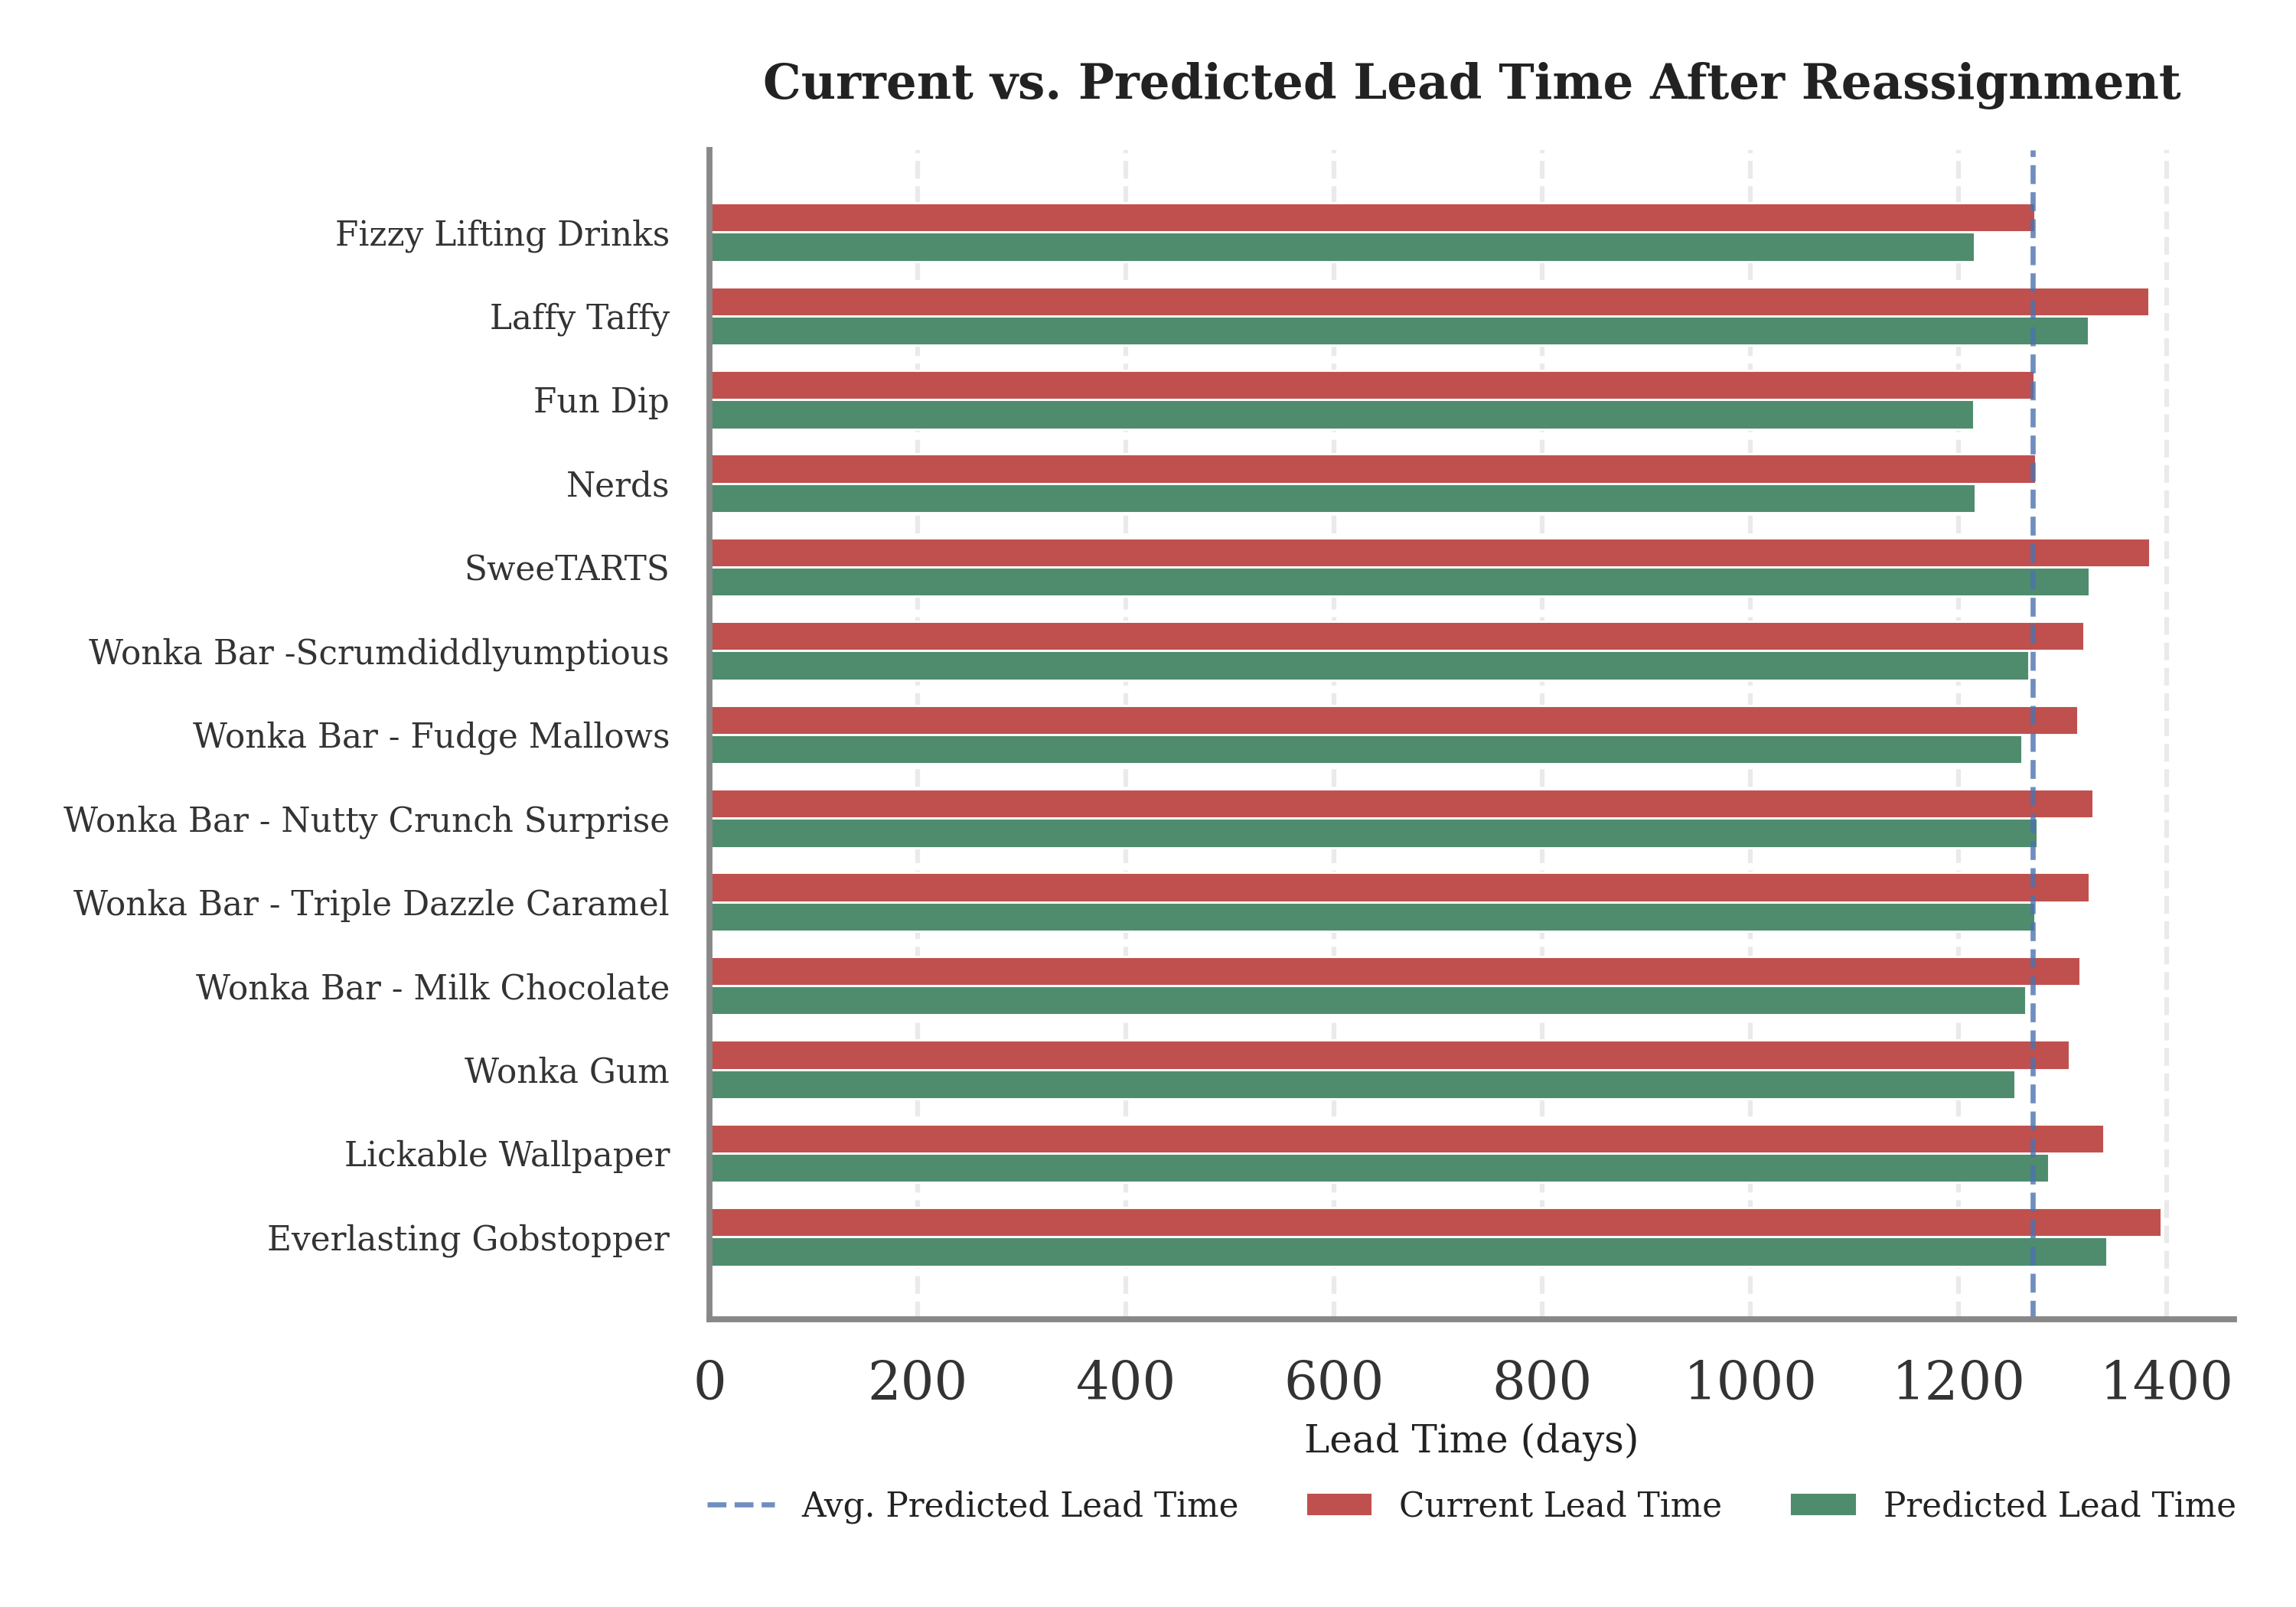
\includegraphics[width=\textwidth]{charts/cvsplead.png}
    \caption{Current vs.\ predicted lead times for all 13
    recommended products after reassignment to The Other
    Factory. Every product records a positive lead time
    reduction; Sugar Shack products benefit most
    (58 days saved).}
    \label{fig:lt_comparison}
\end{figure}
% ------------------------------------------------

% ------------------------------------------------
\begin{figure}[H]
    \centering
    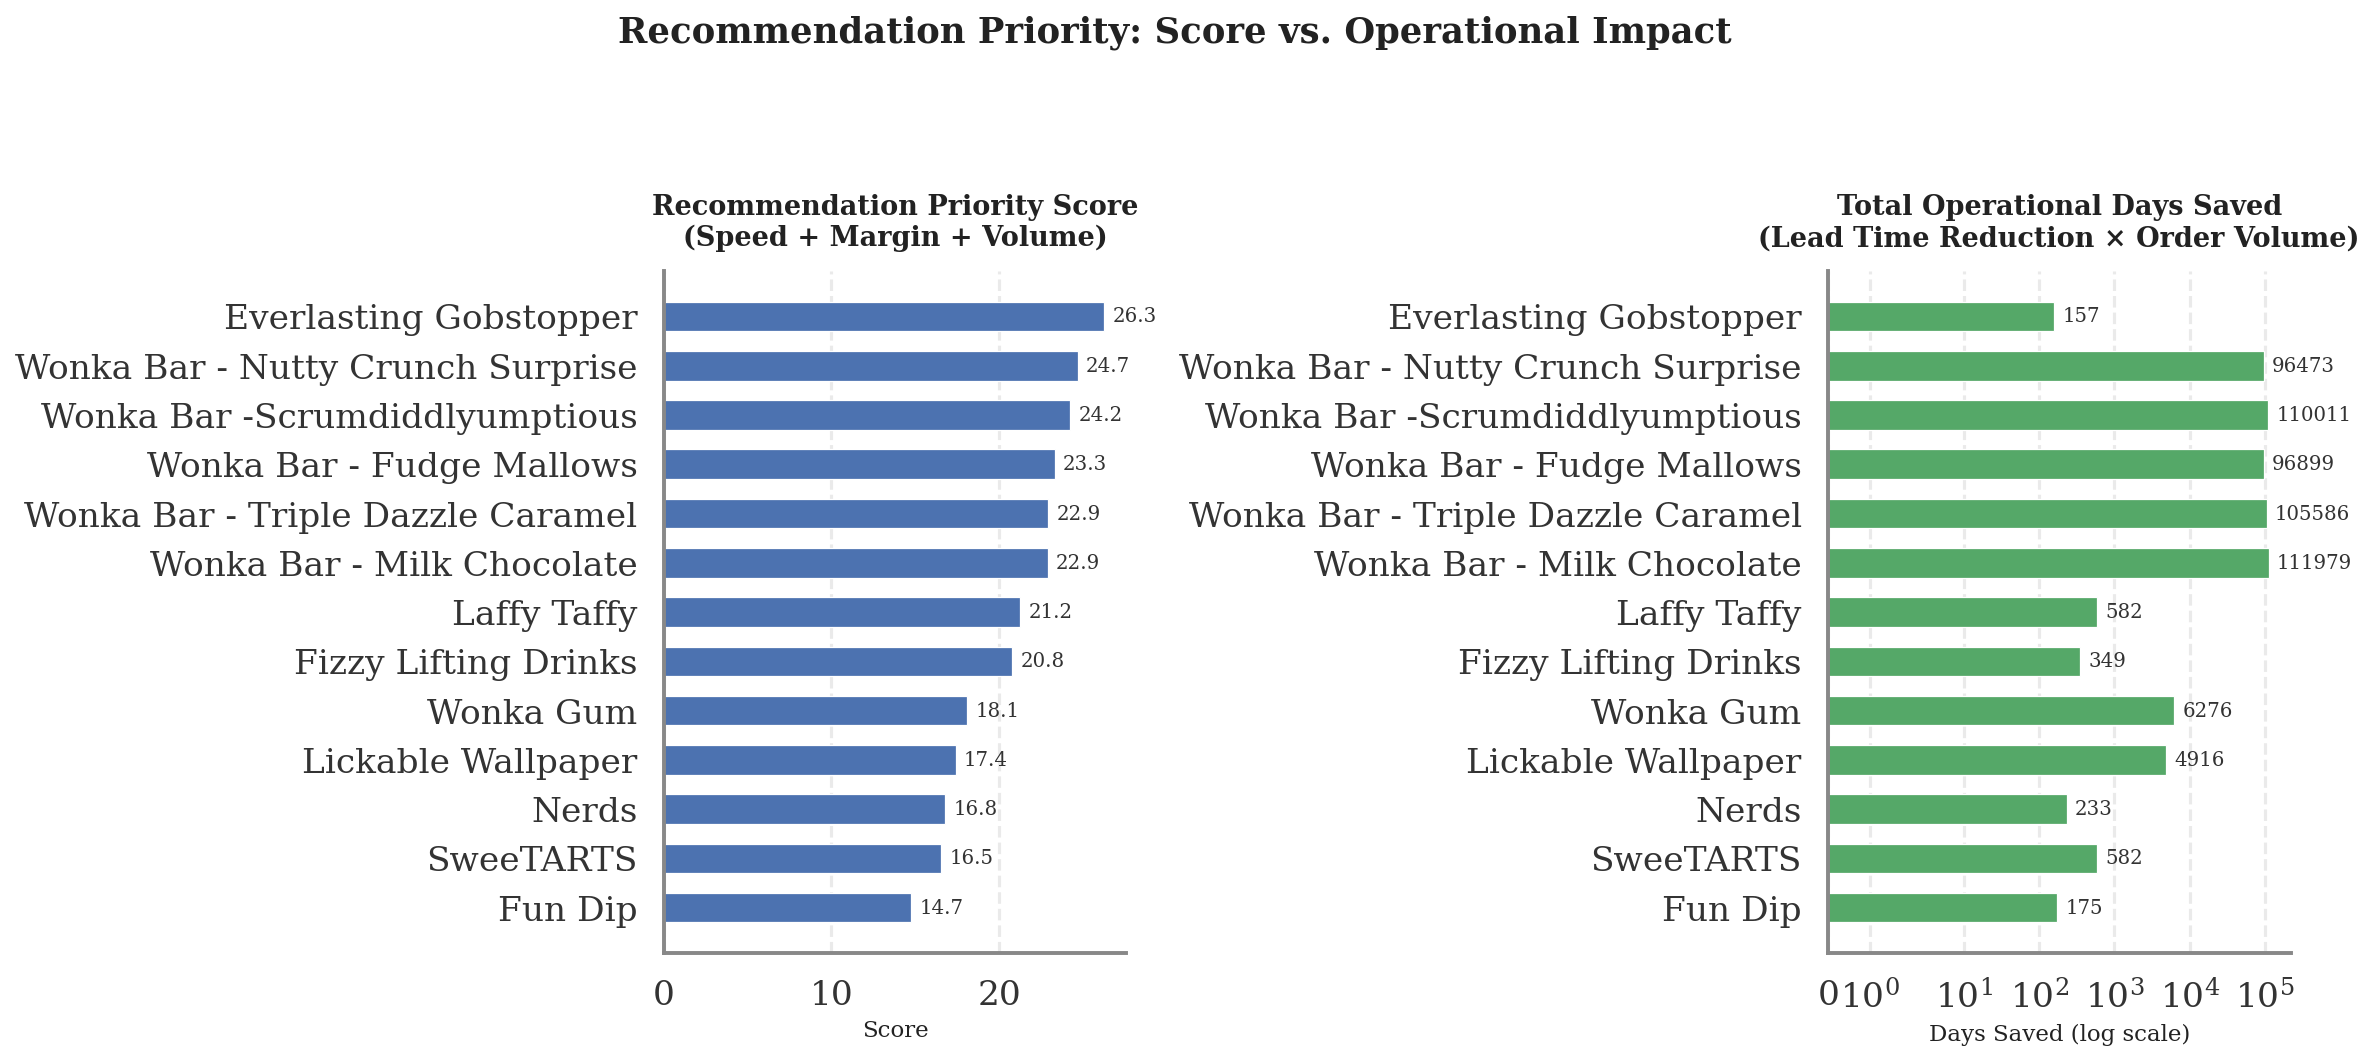
\includegraphics[width=\textwidth]{charts/priorityscore.png}
    \caption{Left: Composite priority scores by product ---
    Everlasting Gobstopper ranks \#1 due to its uniquely
    high profit margin. Right: Total operational days saved
    --- the five Chocolate Wonka Bars dominate due to
    order volume of 1,810--2,137 per product.}
    \label{fig:priority_charts}
\end{figure}
% ------------------------------------------------

% ------------------------------------------------
\begin{figure}[H]
    \centering
    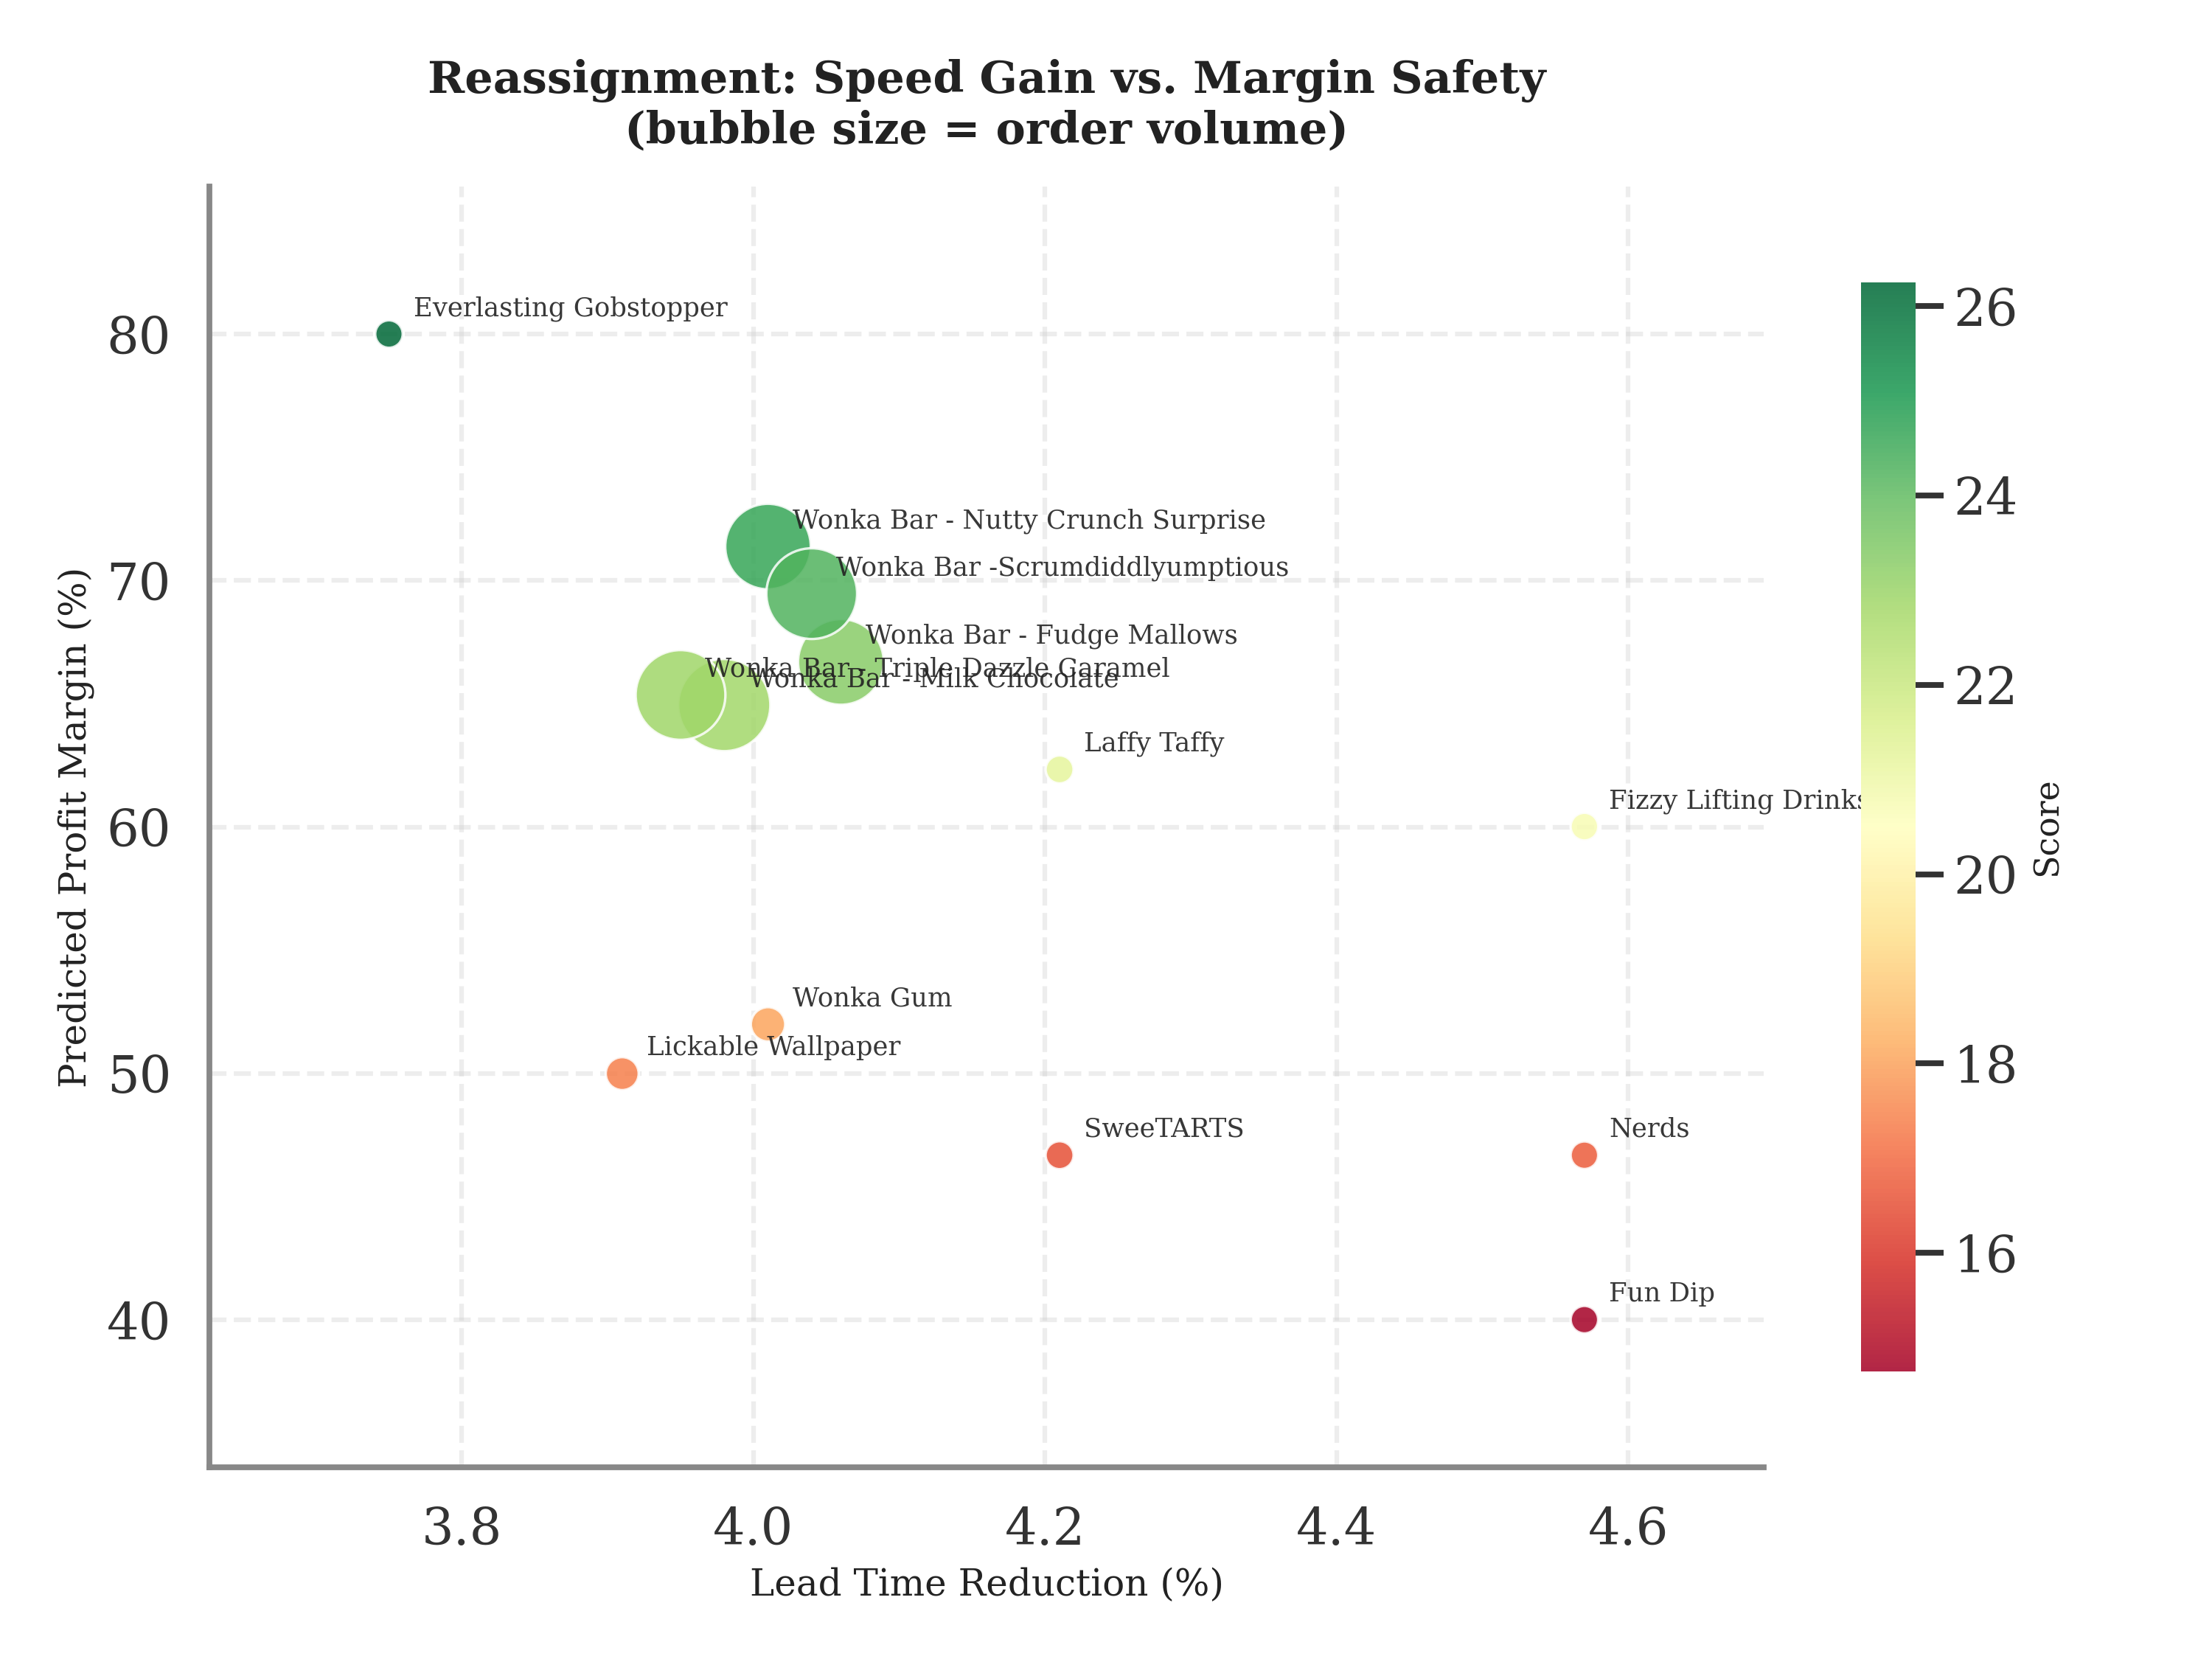
\includegraphics[width=\textwidth]{charts/speednmargin.png}
    \caption{Speed gain (lead time reduction \%) versus
    financial safety (predicted profit margin \%).
    Bubble size represents order volume. Products in the
    upper-right quadrant --- principally the Chocolate Wonka
    Bars --- combine high margin with meaningful speed gains
    and represent the most balanced reassignment candidates.}
    \label{fig:tradeoff}
\end{figure}
% ------------------------------------------------

\subsection{Key Performance Indicators}

Table~\ref{tab:kpis} reports the four KPIs against their
achieved values.

\begin{table}[H]
\centering
\caption{Key Performance Indicators --- Factory
         Reassignment Programme}
\label{tab:kpis}
\renewcommand{\arraystretch}{1.2}
\begin{tabular}{llll}
\toprule
\textbf{KPI} & \textbf{Description} & \textbf{Value}
    & \textbf{Notes} \\
\midrule
Lead Time Reduction (\%)
    & Operational gain
    & 4.24\% avg
    & Range: 3.75\%--4.57\% \\
Profit Impact Stability
    & Financial safety
    & $\Delta < 0.05$ pp
    & Zero products lose margin \\
Scenario Confidence Score
    & Reliability
    & 65.0\%
    & 39 of 60 scenarios improve \\
Recommendation Coverage
    & Scalability
    & 86.7\%
    & 13 of 15 products covered \\
\midrule
\multicolumn{2}{l}{Total Cumulative Days Saved}
    & 534,218 & All 13 products \\
\multicolumn{2}{l}{Avg Reduction per Product}
    & 54.8 days & \\
\bottomrule
\end{tabular}
\end{table}

A clarification is warranted regarding the Scenario Confidence
Score. The 65\% figure (39 of 60 tested scenarios showing lead
time improvement) reflects the full breadth of the simulation
exercise: every feasible product--factory pair was evaluated,
including combinations in which the alternative factory is
objectively slower than the product's current assignment ---
for instance, routing a Lot's O' Nuts product to Wicked
Choccy's, which carries a comparable or higher average lead
time. The 21 non-improving scenarios therefore represent
suboptimal destinations that the scoring framework correctly
eliminates from the final recommendations; they do not
constitute failures of the analysis. The claim that The Other
Factory is the \emph{universally optimal} destination for all
13 products is based solely on the top-scoring scenario per
product, each of which yields a positive lead time reduction
and identifies The Other Factory as the clear winner. The
Scenario Confidence Score characterises the width of the
simulation space, not the quality of the selected
recommendations.

% ============================================================
\section{Conclusion}
\label{sec:conclusion}
% ============================================================

This study conducted a comprehensive data-driven analysis of
Nassau Candy Distributor's order fulfilment operations using
a dataset of 10,194 records spanning 2024--2025. The analysis
proceeded through exploratory data analysis, correlation
analysis, predictive modelling, route and product clustering,
and factory reassignment simulation --- covering every stage of
the analytical methodology specified in the project brief.

The principal findings are as follows:

\begin{enumerate}[leftmargin=*, label=\arabic*.]
    \item \textbf{Lead time variation is primarily temporal.}
          Order Year ($r = 0.72$) is the single dominant
          predictor of lead time, with factory identity
          contributing zero independent predictive power in
          the modelling framework. This finding establishes
          that predictive modelling alone is insufficient as
          an optimisation tool, and motivates the use of
          a simulation-based recommendation engine.
    \item \textbf{Factory capacity is critically imbalanced.}
          Lot's O' Nuts and Wicked Choccy's absorb 96.5\%
          of all orders despite being classified as Congested
          Routes. The Other Factory handles only 1\% of
          volume despite being the fastest factory in the
          network --- the most significant structural
          inefficiency identified in the dataset.
    \item \textbf{The Other Factory is the universal optimal
          reassignment destination.} Simulating all feasible
          reassignment scenarios across 13 products, every
          product's best reassignment is to The Other Factory,
          projecting \textbf{534,218 cumulative operational
          days saved} at an average reduction of
          \textbf{54.8 days per product}.
    \item \textbf{Reassignment is financially safe.} No
          product loses more than 0.05 percentage points of
          profit margin following reassignment. Ten of
          thirteen products are classified as LOW RISK;
          zero are HIGH RISK.
    \item \textbf{Hair Toffee is a special case.} Already
          manufactured at The Other Factory, Hair Toffee's
          unusually high lead time (approximately 1,455 days)
          cannot be addressed through factory reassignment
          and requires a dedicated operational investigation
          (see Appendix~A).
    \item \textbf{Everlasting Gobstopper is the
          highest-priority product by composite score.} Its
          combination of an 80\% profit margin and a
          1,394-day lead time produces the highest priority
          score in the simulation framework, despite only
          3 historical orders.
\end{enumerate}

The practical implication is clear. Nassau Candy should
initiate a phased programme to \textbf{expand The Other
Factory's fulfilment capacity} and systematically transfer
product assignments away from Lot's O' Nuts and Wicked
Choccy's. A recommended phasing sequence is:

\begin{enumerate}[leftmargin=*, label=\textbf{Phase \arabic*.}]
    \item \textbf{Immediate priority --- highest composite
          score:} Everlasting Gobstopper (Secret Factory
          $\rightarrow$ The Other Factory). Highest margin
          in the network; 52 days saved per order.
    \item \textbf{Short-term priority --- highest total days
          saved:} The five Chocolate division Wonka Bars
          (from Lot's O' Nuts and Wicked Choccy's). These
          account for over 480,000 of the projected 534,218
          days saved due to their order volumes of
          1,810--2,137 per product.
    \item \textbf{Medium-term --- remaining products:} Sugar
          Shack and Secret Factory products (Laffy Taffy,
          SweeTARTS, Nerds, Wonka Gum, Lickable Wallpaper,
          Fizzy Lifting Drinks, Fun Dip), pending capacity
          availability at The Other Factory.
\end{enumerate}

\subsection*{Limitations and Future Work}

The following limitations should be addressed in subsequent
analyses:

\begin{itemize}[leftmargin=*]
    \item \textbf{Capacity constraints not modelled.}
          The simulation assumes The Other Factory has
          unlimited capacity to absorb reassigned products.
          In practice, a capacity ceiling will exist.
          Future work should incorporate factory throughput
          constraints to determine the maximum feasible
          reassignment volume and optimise the phasing
          sequence accordingly.
    \item \textbf{Synthetic lead time structure.} The
          dataset's forward-projected ship dates mean that
          absolute lead time values are operationally
          atypical. Results should be validated against
          real-world shipping logs before implementation.
    \item \textbf{Financial sustainability of The Other
          Factory's current product line.} Hair Toffee and
          Kazookles carry approximately 10\% margins. A
          separate pricing or product-mix review is
          warranted independently of the reassignment
          programme.
    \item \textbf{Root cause of Hair Toffee's anomalous
          lead time.} This requires factory-level capacity
          data and product-specific shipping logs beyond
          the scope of the current dataset.
    \item \textbf{Shipping cost data.} Incorporating actual
          freight costs rather than Haversine-estimated
          distances would sharpen the financial dimension
          of the routing recommendations.
\end{itemize}

% ============================================================
% REFERENCES
% ============================================================
\bibliographystyle{apalike}
\begin{thebibliography}{9}

\bibitem[Breiman(2001)]{breiman2001}
Breiman, L. (2001).
Random forests.
\textit{Machine Learning}, \textit{45}(1), 5--32.

\bibitem[Chopra and Meindl(2007)]{chopra2007}
Chopra, S., \& Meindl, P. (2007).
\textit{Supply chain management: Strategy, planning, and operation}
(3rd ed.). Pearson Prentice Hall.

\bibitem[Dantzig and Ramser(1959)]{dantzig1959}
Dantzig, G.~B., \& Ramser, J.~H. (1959).
The truck dispatching problem.
\textit{Management Science}, \textit{6}(1), 80--91.

\bibitem[Farahani et al.(2011)]{farahani2011}
Farahani, R.~Z., Rezapour, S., \& Kardar, L. (Eds.). (2011).
\textit{Logistics operations and management: Concepts and models}.
Elsevier.

\bibitem[Friedman(2001)]{friedman2001}
Friedman, J.~H. (2001).
Greedy function approximation: A gradient boosting machine.
\textit{Annals of Statistics}, \textit{29}(5), 1189--1232.

\bibitem[MacQueen(1967)]{macqueen1967}
MacQueen, J. (1967).
Some methods for classification and analysis of multivariate
observations.
In \textit{Proceedings of the Fifth Berkeley Symposium on
Mathematical Statistics and Probability} (Vol.~1, pp.~281--297).
University of California Press.

\bibitem[Rousseeuw(1987)]{rousseeuw1987}
Rousseeuw, P.~J. (1987).
Silhouettes: A graphical aid to the interpretation and validation
of cluster analysis.
\textit{Journal of Computational and Applied Mathematics},
\textit{20}, 53--65.

\bibitem[Sinnott(1984)]{sinnott1984}
Sinnott, R.~W. (1984).
Virtues of the Haversine.
\textit{Sky and Telescope}, \textit{68}(2), 159.

\end{thebibliography}

% ============================================================
% APPENDICES
% ============================================================
\newpage
\appendix

\section*{Appendix A --- Hair Toffee Analysis Note}
\addcontentsline{toc}{section}{Appendix A --- Hair Toffee Analysis Note}

Hair Toffee records the highest average lead time in the
dataset (approximately 1,455 days) and is classified as
\emph{Slow \& Risky} in the product clustering. It is
manufactured at \textbf{The Other Factory}, which achieves
an overall average lead time of 1,267.3 days across its
100 orders --- the best factory average in the network.

Hair Toffee's lead time of 1,455 days therefore represents
a \textbf{188-day excess relative to its own factory's
average} --- an anomaly that cannot be resolved by
reassignment since The Other Factory is already the optimal
destination. Plausible explanations include:

\begin{itemize}[leftmargin=*]
    \item \textbf{Geographic misalignment:} The Other
          Factory is located at approximately
          35.12\textdegree N, 89.97\textdegree W
          (Memphis, Tennessee area).
          If Hair Toffee demand is concentrated in
          distant regions (e.g.\ Pacific), the shipping
          distance penalty may exceed what regional
          averages capture.
    \item \textbf{Order cohort effects:} Hair Toffee has
          only 4 recorded orders. If these orders were
          placed disproportionately in early 2024
          (the highest lead-time cohort), the product
          average would be inflated.
    \item \textbf{Internal production scheduling:}
          Hair Toffee may require specialised equipment
          or longer production runs at The Other Factory
          relative to Kazookles.
    \item \textbf{Capacity competition:} With only two
          products, any internal prioritisation of
          Kazookles (96 of 100 orders) may create
          scheduling delays for Hair Toffee.
\end{itemize}

\textbf{Recommended action:} A targeted investigation
combining factory capacity logs, product-level shipping
records, and demand geography analysis is required before
any strategic decisions regarding Hair Toffee are made.

\section*{Appendix B --- Computational Environment}
\addcontentsline{toc}{section}{Appendix B --- Computational Environment}

All analysis was conducted in \textbf{Google Colab} using
\textbf{Python 3.12.13}. Package versions are listed in
Table~\ref{tab:packages}. Random states of 42 were used
throughout for reproducibility. The Haversine distance
formula was implemented manually using NumPy without
external geospatial libraries.

\begin{table}[H]
\centering
\caption{Python Package Versions}
\label{tab:packages}
\renewcommand{\arraystretch}{1.15}
\begin{tabular}{ll}
\toprule
\textbf{Package} & \textbf{Version} \\
\midrule
Python        & 3.12.13 \\
pip           & 24.1.2 \\
pandas        & 2.2.2 \\
numpy         & 2.0.2 \\
matplotlib    & 3.10.0 \\
seaborn       & 0.13.2 \\
scikit-learn  & (Colab default for Python 3.12) \\
\bottomrule
\end{tabular}
\end{table}

\begin{lstlisting}[language=Python,
                   caption={Key Libraries Used}]
import pandas as pd
import numpy as np
import matplotlib.pyplot as plt
import seaborn as sns
from sklearn.preprocessing import (
    LabelEncoder, MinMaxScaler, StandardScaler)
from sklearn.model_selection import train_test_split
from sklearn.linear_model import LinearRegression
from sklearn.ensemble import (
    RandomForestRegressor, GradientBoostingRegressor)
from sklearn.metrics import (
    mean_squared_error, mean_absolute_error, r2_score)
from sklearn.cluster import KMeans
from sklearn.metrics import silhouette_score
# Haversine formula implemented manually via NumPy
\end{lstlisting}

% ============================================================
\end{document}
% ============================================================